\section{Preliminaries}\label{sect:prelim}

In this section, we review the basics of matrix Schubert varieties as well as the CDG generators introduced in \cite{HPW}.  For a more detailed introduction to matrix Schubert varieties, we refer the reader to \cite[Chapter 10]{Ful96}.  For basic properties of and standard terminology for Gr\"obner bases, we refer the reader to \cite{Eis95}.  

\subsection{Matrix Schubert varieties}\label{subsect:MSv}

We begin by describing how each permutation is associated to the affine variety called a matrix Schubert variety.  Throughout this paper, we will take  $[n] = \{1,2,\dots,n\}$  for any $n \geq 1$ and let $S_n$ denote the symmetric group on $[n]$.  Each permutation $w \in S_n$ is a bijection $w:[n] \rightarrow [n]$, which we will record in its one-line notation $w = w_1 w_2 \dots w_n$ where $w_i = w(i)$.  To every $w \in S_n$, we associate a \emph{Rothe diagram} $D_w$, defined as follows:
\[
D_w = \{(i,j) \in [n] \times [n]: w(i) > j, w^{-1}(j) > i\}.
\]
A Rothe diagram has the following visualization: In an $n \times n$ grid, place a $\bullet$ in position $(i,w_i)$ for each $i \in [n]$, and draw a line down from each $\bullet$ to the bottom of the grid and a line to the right from each $\bullet$ to the side of the grid.  Then $D_w$ is the set of boxes in the grid without a $\bullet$ in them or a line through them.
For example, $D_{315642}$ is the set $\{(1,1),(1,2),(3,2),(3,4),(4,2),(4,4),(5,2)\}$ and corresponds to the visualization below, in which the elements of $D_{315642}$ appear in gray and will be referred to as the \emph{boxes} of $w$:
\[
  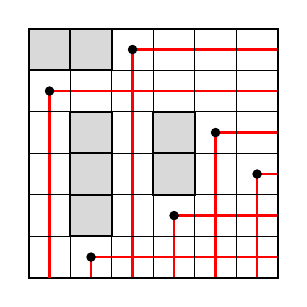
\begin{tikzpicture}[x=1.5em,y=1.5em]
      \draw[color=black, thick](0,1)rectangle(6,7);
     \filldraw[color=black, fill=gray!30, thick](0,6)rectangle(1,7);
      \filldraw[color=black, fill=gray!30, thick](1,6)rectangle(2,7);
      \filldraw[color=black, fill=gray!30, thick](1,4)rectangle(2,5);
      \filldraw[color=black, fill=gray!30, thick](3,4)rectangle(4,5);
       \filldraw[color=black, fill=gray!30, thick](1,3)rectangle(2,4);
      \filldraw[color=black, fill=gray!30, thick](3,3)rectangle(4,4);
      \filldraw[color=black, fill=gray!30, thick](1,2)rectangle(2,3);      
     \draw[thick,color=red] (6,6.5)--(2.5,6.5)--(2.5,1);
     \draw[thick,color=red] (6,5.5)--(0.5,5.5)--(0.5,1);
     \draw[thick,color=red] (6,4.5)--(4.5,4.5)--(4.5,1);
     \draw[thick,color=red] (6,3.5)--(5.5,3.5)--(5.5,1);
     \draw[thick,color=red] (6,2.5)--(3.5,2.5)--(3.5,1);
     \draw[thick,color=red] (6,1.5)--(1.5,1.5)--(1.5,1);
     \filldraw [black](2.5,6.5)circle(.1);
     \filldraw [black](0.5,5.5)circle(.1);
      \filldraw [black](4.5,4.5)circle(.1);
     \filldraw [black](5.5,3.5)circle(.1);
     \filldraw [black](3.5,2.5)circle(.1);
      \filldraw [black](1.5,1.5)circle(.1);
      \draw[color=black](2,6)rectangle(3,7);
      \draw[color=black](3,6)rectangle(4,7); 
      \draw[color=black](4,6)rectangle(5,7);
      \draw[color=black](5,6)rectangle(6,7); 
      \draw[color=black](0,5)rectangle(1,6);
      \draw[color=black](1,5)rectangle(2,6);  
      \draw[color=black](2,5)rectangle(3,6);
      \draw[color=black](3,5)rectangle(4,6); 
      \draw[color=black](4,5)rectangle(5,6);
      \draw[color=black](5,5)rectangle(6,6); 
     \draw[color=black](0,4)rectangle(1,5); 
      \draw[color=black](2,4)rectangle(3,5);
      \draw[color=black](4,4)rectangle(5,5);
      \draw[color=black](5,4)rectangle(6,5); 
      \draw[color=black](0,3)rectangle(1,4); 
      \draw[color=black](2,3)rectangle(3,4);
      \draw[color=black](4,3)rectangle(5,4);
      \draw[color=black](5,3)rectangle(6,4); 
      \draw[color=black](0,2)rectangle(1,3); 
      \draw[color=black](2,2)rectangle(3,3);
      \draw[color=black](3,2)rectangle(4,3);
      \draw[color=black](4,2)rectangle(5,3);
      \draw[color=black](5,2)rectangle(6,3); 
      \draw[color=black](1,1)rectangle(2,2);  
      \draw[color=black](2,1)rectangle(3,2);
      \draw[color=black](3,1)rectangle(4,2); 
      \draw[color=black](4,1)rectangle(5,2);
      \draw[color=black](5,1)rectangle(6,2); 
     \end{tikzpicture}.
\]

The \emph{Coxeter length} of the permutation $w$ is equal to its inversion number, i.e. 
\[| \{ (i, j) \mid i < j, w_i > w_j \}|,
\] which is in turn equal to $|D_w|$.  For example, the Coxeter length of $315642$ is $7$, easily read off as the number of gray boxes in the diagram above.

\begin{definition}
Fix a permutation $w = w_1 \cdots w_n \in S_n$ and a permutation $v  = v_1\ldots v_k \in S_k$ with $k \leq n$.  If there is some substring $w_{i_1} \cdots w_{i_k}$ of $w$ satisfying $w_{i_j} < w_{i_\ell}$ exactly when $v_j < v_\ell$, then we say that $w$ \emph{contains} $v$.  Otherwise, we say that $w$ \emph{avoids} $v$.
\end{definition}

For example, $w = 13254$ contains $v = 2143$ with $3254$ the substring of $w$ realizing the containment, but $w$ does not contain $v' = 3214$.  Notice that if $w_{i_1} \cdots w_{i_k}$ satisfies $w_{i_j} < w_{i_\ell}$ exactly when $v_j < v_\ell$, then the Rothe diagram of $v$ can be obtained from that of $w$ by restricting to the rows $i_1, \ldots, i_k$ and columns $w_{i_1}, \ldots, w_{i_k}$ in the $[n] \times [n]$ grid giving the visualization of $D_w$.  

By restricting to the maximally southeast boxes of connected components of $D_w$, we define the \emph{essential set} of $w$: 
\[
\Ess(w) = \{(i,j) \in D_w \mid (i+1,j), (i,j+1) \notin D_w\}.
\]
In the example above, $\Ess(315642)=\{(1,2),(4,4), (5,2)\}$.  Borrowing a term from the literature on ladder determinantal varieties, if $(i,j) \in \Ess(w)$ and there is no $(i'j') \in \Ess(w)$ with $i \leq i'$, $j \leq j'$, and $(i,j) \neq (i',j')$, we will say that $(i,j)$ is a \emph{lower outside corner} of $D_w$.  In the case of $w = 315642$, $(4,4)$ and $(5,2)$ are lower outside corners, but $(1,2)$ is not.  

To every permutation $w \in S_n$, we associate a \emph{rank function} $\rank_w : [n] \times [n] \to \mathbb{Z}$, where 
\[
\rank_w(i,j) = |\{k \leq i \mid w(k) \leq j\}|,
\] and the rank matrix $M_w$ whose $(i,j)^{th}$ entry is $\rank_w(i,j)$.  Visually, we assign to every square $(i,j)$ in the $[n] \times [n]$ grid underlying the Rothe diagram of $w$ the number of $\bullet$s weakly northwest of $(i,j)$.  In our running example $w = 315642$, one may find it helpful to record the information as  \definecolor{burntorange}{rgb}{0.8, 0.33, 0.0}
\[
\begin{minipage}{0.4\textwidth}\
\[
\hspace{1cm} M_w = \begin{bmatrix}
\boxed{0} & {\color{burntorange}\boxed{0}} & 1 & 1 & 1 & 1\\
1 & 1 & 2 & 2 & 2 & 2\\
1 & \boxed{1} & 2 & \boxed{2} & 3 & 3\\
1 & \boxed{1} & 2 & {\color{burntorange}\boxed{2}} & 3 & 4\\
1 & {\color{burntorange}\boxed{1}} & 2 & 3 & 4 & 5\\
1 & 2 & 3 & 4 & 5 & 6\\
\end{bmatrix} 
\]

\end{minipage} \hspace{1cm} \mbox{ or as } \hspace{0.6cm} \begin{minipage}{.4\textwidth}
\hspace{0.5cm} 
  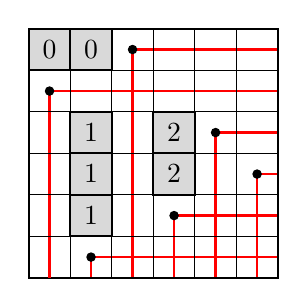
\begin{tikzpicture}[x=1.5em,y=1.5em]
      \draw[color=black, thick](0,1)rectangle(6,7);
     \filldraw[color=black, fill=gray!30, thick](0,6)rectangle(1,7);
      \filldraw[color=black, fill=gray!30, thick](1,6)rectangle(2,7);
      \filldraw[color=black, fill=gray!30, thick](1,4)rectangle(2,5);
      \filldraw[color=black, fill=gray!30, thick](3,4)rectangle(4,5);
       \filldraw[color=black, fill=gray!30, thick](1,3)rectangle(2,4);
      \filldraw[color=black, fill=gray!30, thick](3,3)rectangle(4,4);
      \filldraw[color=black, fill=gray!30, thick](1,2)rectangle(2,3);      
     \draw[thick,color=red] (6,6.5)--(2.5,6.5)--(2.5,1);
     \draw[thick,color=red] (6,5.5)--(0.5,5.5)--(0.5,1);
     \draw[thick,color=red] (6,4.5)--(4.5,4.5)--(4.5,1);
     \draw[thick,color=red] (6,3.5)--(5.5,3.5)--(5.5,1);
     \draw[thick,color=red] (6,2.5)--(3.5,2.5)--(3.5,1);
     \draw[thick,color=red] (6,1.5)--(1.5,1.5)--(1.5,1);
     \filldraw [black](2.5,6.5)circle(.1);
     \filldraw [black](0.5,5.5)circle(.1);
      \filldraw [black](4.5,4.5)circle(.1);
     \filldraw [black](5.5,3.5)circle(.1);
     \filldraw [black](3.5,2.5)circle(.1);
      \filldraw [black](1.5,1.5)circle(.1);
      \draw[color=black](2,6)rectangle(3,7);
      \draw[color=black](3,6)rectangle(4,7); 
      \draw[color=black](4,6)rectangle(5,7);
      \draw[color=black](5,6)rectangle(6,7); 
      \draw[color=black](0,5)rectangle(1,6);
      \draw[color=black](1,5)rectangle(2,6);  
      \draw[color=black](2,5)rectangle(3,6);
      \draw[color=black](3,5)rectangle(4,6); 
      \draw[color=black](4,5)rectangle(5,6);
      \draw[color=black](5,5)rectangle(6,6); 
     \draw[color=black](0,4)rectangle(1,5); 
      \draw[color=black](2,4)rectangle(3,5);
      \draw[color=black](4,4)rectangle(5,5);
      \draw[color=black](5,4)rectangle(6,5); 
      \draw[color=black](0,3)rectangle(1,4); 
      \draw[color=black](2,3)rectangle(3,4);
      \draw[color=black](4,3)rectangle(5,4);
      \draw[color=black](5,3)rectangle(6,4); 
      \draw[color=black](0,2)rectangle(1,3); 
      \draw[color=black](2,2)rectangle(3,3);
      \draw[color=black](3,2)rectangle(4,3);
      \draw[color=black](4,2)rectangle(5,3);
      \draw[color=black](5,2)rectangle(6,3); 
      \draw[color=black](1,1)rectangle(2,2);  
      \draw[color=black](2,1)rectangle(3,2);
      \draw[color=black](3,1)rectangle(4,2); 
      \draw[color=black](4,1)rectangle(5,2);
      \draw[color=black](5,1)rectangle(6,2); 
     \node at (0.5,6.5) {$0$};
      \node at (1.5,6.5) {$0$};
      \node at (1.5,4.5) {$1$};
      \node at (1.5,3.5) {$1$};
      \node at (1.5,2.5) {$1$};
       \node at (3.5,4.5) {$2$};
       \node at (3.5,3.5) {$2$};
     \end{tikzpicture}.
  \end{minipage}   
       \]
Note that the transpose of the rank matrix of $w$ and transpose of the Rothe diagram of $w$ correspond to the rank matrix and Rothe diagram of $w^{-1}$, respectively, because the inverse of a permutation matrix is its transpose.  We have recorded elements of $D_w$ in the rank matrix $M_w$ as boxes and colored the boxes of the essential set orange in anticipation of our discussion of Fulton generators, below.

Let $\mbox{Mat}_{n,n}$ denote the affine $n^2$-space of complex $n \times n$ matrices.  Given $N \in \mbox{Mat}_{n,n}$ and subsets $A,B \subseteq [n]$, let $N_{A,B}$ be the submatrix of $N$ determined by the rows whose indices are elements of $A$ and the columns whose indices are elements of $B$.  Then the \emph{matrix Schubert variety} of $w \in S_n$ is the affine variety \[
X_w = \left\{Z \in \mbox{Mat}_{n,n}\mid \rank{Z_{[i],[j]}} \leq \rank_w(i,j)\ \mbox{for all}\ (i,j) \in [n] \times [n] \right\}.
\]

Let $Z = (z_{i,j})_{(i,j) \in [n] \times [n]}$ be a matrix of distinct indeterminates and $R = \mathbb{C}[Z]$ so that $\Spec(R)$ is identified with $\mbox{Mat}_{n,n}$.  The \emph{Schubert determinantal ideal} of $w$ is 
\[
I_w = ( (\rank_w(i,j)+1)\text{-minors in } Z_{[i],[j]} \mid (i,j) \in [n] \times [n] ) \subseteq R.
\]  This naive generating set will typically include a good deal of redundancy, and so we will more often consider the smaller set of \emph{Fulton generators} of $I_w$: \[
	\{(\rank_w(i,j)+1)\text{-minors in } Z_{[i],[j]} \mid (i,j) \in \Ess(w) \}.
\]  Fulton showed that the Fulton generators indeed generate $I_w$ \cite[Lemma 3.10]{Ful92}, that $I_w$ is prime, and, in particular, that $X_w \cong \Spec(R/I_w)$ as reduced schemes  \cite[Proposition 3.3]{Ful92}.  The height of the ideal $I_w$ (equivalently, codimension of $\Spec(R/I_w)$ in $\Spec(R)$) is equal to the Coxeter length of $w$ \cite[Proposition 3.3]{Ful92}.

In the example $w = 315642$, the Fulton generators of $I_w$ are $z_{1,1}$, $z_{1,2}$, the $2$-minors of \begin{center} $\begin{bmatrix}
z_{1,1} & z_{1,2}\\
z_{2,1} & z_{2,2}\\
z_{3,1} & z_{3,2}\\
z_{4,1} & z_{4,2}\\
z_{5,1} & z_{5,2}\\
\end{bmatrix},
$ and the $3$-minors of  $\begin{bmatrix}
z_{1,1} & z_{1,2} & z_{1,3} & z_{1,4}\\
z_{2,1} & z_{2,2} & z_{2,3} & z_{2,4}\\
z_{3,1} & z_{3,2} & z_{3,3} & z_{3,4}\\
z_{4,1} & z_{4,2} & z_{4,3} & z_{4,4}\\
\end{bmatrix}.
$ \end{center} 

\subsection{CDG generators}\label{subsect:CDG}

In \cite{HPW}, the authors introduce \emph{CDG generators} of defining ideals of matrix Schubert varieties.  These generators are named after Conca, De Negri, and Gorla, whose result \cite[Theorem 4.2]{CDG15} served as inspiration for the generating set used in \cite{HPW} and, in particular, for Conjecture \ref{conj:mainresult}.

\begin{definition}
Fix a permutation $w \in S_n$ and an $n \times n$ matrix $Z = (z_{i,j})_{(i,j) \in [n] \times [n]}$ of distinct indeterminates.  Let $\Dom(w) = \{(i,j) \in D_w \mid \rank_w(i,j) = 0\}$, and call $\Dom(w)$ the \emph{dominant part} of the Rothe diagram $D_w$.  From $Z$, form the matrix $Z'$ by replacing $z_{i,j}$ by $0$ whenever $(i,j) \in \Dom(w)$.  Set \[
	G'_w = \{(\rank_w(i,j)+1)\text{-minors in } Z'_{[i],[j]} \mid (i,j) \in \Ess(w)\setminus \Dom(w) \},
\] and $G_w = G'_w \cup \{z_{i,j} \mid (i,j) \in \Dom(w)\}$.  We call $G_w$ the set of \emph{CDG generators} of $I_w$.
\end{definition}

\begin{example}
If $w = 315642$ the CDG generators of $I_w$ are $z_{1,1}$, $z_{1,2}$, the $2$-minors of \begin{center} $\begin{bmatrix}
0 & 0\\
z_{2,1} & z_{2,2}\\
z_{3,1} & z_{3,2}\\
z_{4,1} & z_{4,2}\\
z_{5,1} & z_{5,2}\\
\end{bmatrix},
$ and the $3$-minors of  $\begin{bmatrix}
0 & 0 & z_{1,3} & z_{1,4}\\
z_{2,1} & z_{2,2} & z_{2,3} & z_{2,4}\\
z_{3,1} & z_{3,2} & z_{3,3} & z_{3,4}\\
z_{4,1} & z_{4,2} & z_{4,3} & z_{4,4}\\
\end{bmatrix}.
$ \end{center}
\end{example}

\noindent Notice that $\Dom(w) = \emptyset$ if and only if $w_1 = 1$, in which case the CDG generators and the Fulton generators coincide.  

\subsection{Gr\"obner bases}\label{subsect:Grobner}

Let $S=\mathbb{C}[x_1, \ldots, x_d]$.  A \emph{term order} $<$ on $S$ is a total order on the monic monomials of $S$ so that $1 \leq \mu$ for every monomial $\mu$ of $S$ and so that, for all monomials $\mu_1, \mu_2$, and $\nu$, $\mu_1<\mu_2$ implies $\mu_1 \nu < \mu_2 \nu$.  Let $f = \sum_{i=1}^k c_i \mu_i \in S$ where $c_i \in \CC$ and the $\mu_i$ are monic monomials (written in the usual way so that $\mu_i \neq \mu_j$ whenever $i \neq j$ and no $c_i$ is  $0$).  Fix $i$ so that $c_i \mu_i >c_j \mu_j$ whenever $i \neq j$, and define the \emph{leading term} of $f$ to be $LT(f)=c_i \mu_i$.  For an ideal $I$ of $S$, define the \emph{initial ideal} of $I$ to be $LT(I) = (LT(f) \mid f \in I)$.  A generating set $\mathcal{G}$ of $I$ is called a \emph{Gr\"obner basis} if $LT(I) = (LT(g) \mid g \in \mathcal{G})$.  For a detailed introduction to the theory of Gr\"obner bases, including Buchberger's algorithm, we refer the reader to \cite[Chapter 15]{Eis95}.

\begin{definition}
When the set of CDG generators forms a Gr\"obner basis for the Schubert determinantal ideal $I_w$ under every diagonal term order, we will say that the permutation \emph{$w$ is CDG}.  
\end{definition}

\section{Rothe diagrams of CDG permutations}\label{sect:backward}

\subsection{Obstructions to being CDG}

We begin this section by describing in terms of the Rothe diagram $D_w$ conditions that prevent $w$ from being CDG.  In Subsection \ref{subsect:backward}, we will show that when $D_w$ does not satisfy these conditions, $w$ is necessarily CDG.

Before we begin, we note that the visualization of the Rothe diagram of $214635$ is obtained from that of $215364$ by transposition.  The same is true of $315264$ and $241635$.  The visualizations of the Rothe diagrams of the remaining permutations listed in Conjecture \ref{conj:mainresult} are self transpose.   This symmetry will allow us to consolidate some of our case work below.  We understand the cardinal directions in reference to $D_w$ in terms of its visualization.  We say, for example, that $(i',j')$ is ``strictly southeast" of $(i,j)$ to mean that both $i'>i$ and also $j'>j$, or that $(i',j')$ is ``strictly south and weakly east" of $(i,j)$ to mean $i'>i$ and also $j' \geq j$.

\begin{definition}
The permutation $w$ has an \emph{obstruction} of \begin{itemize}
\item \emph{Type 1} if there is some $(r,s) \in \Dom(w) \cap \Ess(w)$ and two distinct entries $(i,j)$ and $(i',j')$ of $D_w$ strictly southeast of $(r,s)$ with $i' \neq i$ and $j' \neq j$,
\item \emph{Type 2} if there is some $(r,s) \in \Dom(w) \cap \Ess(w)$ and two distinct entries $(i,j)$ and $(i,j')$ of $\Ess(w)$ strictly southeast of $(r,s)$ with \[
\max_k \{(k,j) \in \Dom(w)\} = \max_k \{(k,j') \in \Dom(w)\}
\] or, symmetrically, two distinct entries $(i,j)$ and $(i',j)$ of $\Ess(w)$ strictly southeast of $(r,s)$ with \[
\max_\ell \{(i,\ell) \in \Dom(w)\} = \max_\ell \{(i',\ell) \in \Dom(w)\},
\]
\item \emph{Type 3} if there are two distinct entries $(i,j)$ and $(i',j')$ of $\Ess(w) \setminus \Dom(w)$ with $(i',j')$ strictly southeast of $(i,j)$.\qedhere
\end{itemize}
\end{definition}

\begin{example}

The permutation $321654$ has an obstruction of Type $1$ with $(r,s) = (2,1)$, $(i,j) = (4,5)$ and $(i',j') = (5,4)$.  These three essential boxes are shaded in light grey.

\[
  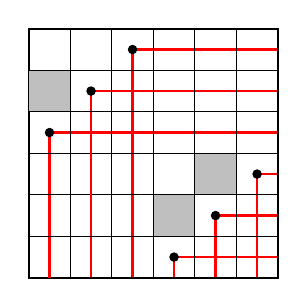
\begin{tikzpicture}[x=1.5em,y=1.5em]
      \draw[color=black, thick](0,1)rectangle(6,7);
      \filldraw [color = lightgray] (0,5)rectangle(1,6);
      \filldraw [color = lightgray] (4,3)rectangle(5,4);
     \filldraw [color = lightgray] (3,2)rectangle(4,3);
     \draw[color=black](0,6)rectangle(1,7);
      \draw[color=black](1,6)rectangle(2,7);
      \draw[color=black](1,4)rectangle(2,5);
      \draw[color=black](3,4)rectangle(4,5);
       \draw[color=black](1,3)rectangle(2,4);
      \draw[color=black](3,3)rectangle(4,4);
      \draw[color=black](1,2)rectangle(2,3);
      \draw[color=black](0,1)rectangle(1,2);        
     \draw[thick,color=red] (6,6.5)--(2.5,6.5)--(2.5,1);
     \draw[thick,color=red] (6,5.5)--(1.5,5.5)--(1.5,1);
     \draw[thick,color=red] (6,4.5)--(0.5,4.5)--(0.5,1);
     \draw[thick,color=red] (6,3.5)--(5.5,3.5)--(5.5,1);
     \draw[thick,color=red] (6,2.5)--(4.5,2.5)--(4.5,1);
     \draw[thick,color=red] (6,1.5)--(3.5,1.5)--(3.5,1);
     \filldraw [black](2.5,6.5)circle(.1);
     \filldraw [black](0.5,4.5)circle(.1);
      \filldraw [black](4.5,2.5)circle(.1);
     \filldraw [black](5.5,3.5)circle(.1);
     \filldraw [black](3.5,1.5)circle(.1);
      \filldraw [black](1.5,5.5)circle(.1);
      \draw[color=black](2,6)rectangle(3,7);
      \draw[color=black](3,6)rectangle(4,7); 
      \draw[color=black](4,6)rectangle(5,7);
      \draw[color=black](5,6)rectangle(6,7); 
      \draw[color=black](0,5)rectangle(1,6);
      \draw[color=black](1,5)rectangle(2,6);  
      \draw[color=black](2,5)rectangle(3,6);
      \draw[color=black](3,5)rectangle(4,6); 
      \draw[color=black](4,5)rectangle(5,6);
      \draw[color=black](5,5)rectangle(6,6); 
     \draw[color=black](0,4)rectangle(1,5); 
      \draw[color=black](2,4)rectangle(3,5);
      \draw[color=black](4,4)rectangle(5,5);
      \draw[color=black](5,4)rectangle(6,5); 
      \draw[color=black](0,3)rectangle(1,4); 
      \draw[color=black](2,3)rectangle(3,4);
      \draw[color=black](4,3)rectangle(5,4);
      \draw[color=black](5,3)rectangle(6,4); 
      \draw[color=black](0,2)rectangle(1,3); 
      \draw[color=black](2,2)rectangle(3,3);
      \draw[color=black](3,2)rectangle(4,3);
      \draw[color=black](4,2)rectangle(5,3);
      \draw[color=black](5,2)rectangle(6,3); 
      \draw[color=black](1,1)rectangle(2,2);  
      \draw[color=black](2,1)rectangle(3,2);
      \draw[color=black](3,1)rectangle(4,2); 
      \draw[color=black](4,1)rectangle(5,2);
      \draw[color=black](5,1)rectangle(6,2); 
     \end{tikzpicture}.
\] 


The permutation $w=4263751$ has an obstruction of Type $2$ with $(r,s) = (1,3)$, $(i,j) = (3,5)$, and $(i,j') = (5,5)$.  These three essential boxes are shaded in light grey.  Here $\max_\ell \{(3,\ell) \in \Dom(w)\} =1= \max_\ell \{(5,\ell) \in \Dom(w)\}$.  

\[
  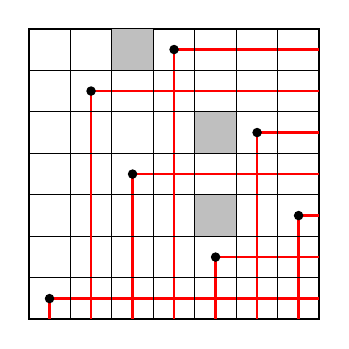
\begin{tikzpicture}[x=1.5em,y=1.5em]
      \draw[color=black, thick](0,1)rectangle(7,8);
      \filldraw [color = lightgray] (2,7)rectangle(3,8);
      \filldraw [color = lightgray] (4,3)rectangle(5,4);
     \filldraw [color = lightgray] (4,5)rectangle(5,6);
     \draw[color=black](0,6)rectangle(1,7);
      \draw[color=black](1,6)rectangle(2,7);
      \draw[color=black](1,4)rectangle(2,5);
      \draw[color=black](3,4)rectangle(4,5);
       \draw[color=black](1,3)rectangle(2,4);
      \draw[color=black](3,3)rectangle(4,4);
      \draw[color=black](1,2)rectangle(2,3);  
       \draw[color=black](0,1)rectangle(1,2);  
      \draw[thick,color=red] (7,7.5)--(3.5,7.5)--(3.5,1);    
     \draw[thick,color=red] (7,6.5)--(1.5,6.5)--(1.5,1);
     \draw[thick,color=red] (7,5.5)--(5.5,5.5)--(5.5,1);
     \draw[thick,color=red] (7,4.5)--(2.5,4.5)--(2.5,1);
     \draw[thick,color=red] (7,3.5)--(6.5,3.5)--(6.5,1);
     \draw[thick,color=red] (7,2.5)--(4.5,2.5)--(4.5,1);
     \draw[thick,color=red] (7,1.5)--(0.5,1.5)--(0.5,1);
     \filldraw [black](0.5,1.5)circle(.1);
     \filldraw [black](2.5,4.5)circle(.1);
      \filldraw [black](4.5,2.5)circle(.1);
     \filldraw [black](5.5,5.5)circle(.1);
     \filldraw [black](3.5,7.5)circle(.1);
      \filldraw [black](1.5,6.5)circle(.1);
       \filldraw [black](6.5,3.5)circle(.1);
      \draw[color=black](2,6)rectangle(3,7);
      \draw[color=black](3,6)rectangle(4,7); 
      \draw[color=black](4,6)rectangle(5,7);
      \draw[color=black](5,6)rectangle(6,7); 
      \draw[color=black](0,5)rectangle(1,6);
      \draw[color=black](1,5)rectangle(2,6);  
      \draw[color=black](2,5)rectangle(3,6);
      \draw[color=black](3,5)rectangle(4,6); 
      \draw[color=black](4,5)rectangle(5,6);
      \draw[color=black](5,5)rectangle(6,6); 
      \draw[color=black](0,4)rectangle(1,5); 
      \draw[color=black](2,4)rectangle(3,5);
      \draw[color=black](4,4)rectangle(5,5);
      \draw[color=black](5,4)rectangle(6,5); 
      \draw[color=black](0,3)rectangle(1,4); 
      \draw[color=black](2,3)rectangle(3,4);
      \draw[color=black](4,3)rectangle(5,4);
      \draw[color=black](5,3)rectangle(6,4); 
      \draw[color=black](0,2)rectangle(1,3); 
      \draw[color=black](2,2)rectangle(3,3);
      \draw[color=black](3,2)rectangle(4,3);
      \draw[color=black](4,2)rectangle(5,3);
      \draw[color=black](5,2)rectangle(6,3); 
      \draw[color=black](1,1)rectangle(2,2);  
      \draw[color=black](2,1)rectangle(3,2);
      \draw[color=black](3,1)rectangle(4,2); 
      \draw[color=black](4,1)rectangle(5,2);
      \draw[color=black](5,1)rectangle(6,2); 
      \draw[color=black](0,7)rectangle(1,8); 
      \draw[color=black](1,7)rectangle(2,8); 
      \draw[color=black](2,7)rectangle(3,8);
      \draw[color=black](3,7)rectangle(4,8);
      \draw[color=black](4,7)rectangle(5,8);
      \draw[color=black](5,7)rectangle(6,8); 
      \draw[color=black](6,7)rectangle(7,8); 
      \draw[color=black](6,1)rectangle(7,2); 
       \draw[color=black](6,2)rectangle(7,3); 
       \draw[color=black](6,3)rectangle(7,4); 
       \draw[color=black](6,4)rectangle(7,5); 
       \draw[color=black](6,5)rectangle(7,6); 
       \draw[color=black](6,6)rectangle(7,7); 
     \end{tikzpicture}.
\]

The permutation $214365$ has an obstruction of Type $3$ with $(i,j) = (3,3)$ and $(i',j') = (5,5)$.  These two essential boxes are shaded in light grey. 

\[
  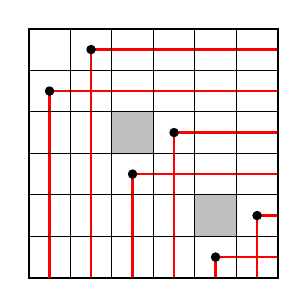
\begin{tikzpicture}[x=1.5em,y=1.5em]
      \draw[color=black, thick](0,1)rectangle(6,7);
     \filldraw [color = lightgray] (4,2)rectangle(5,3);
     \filldraw [color = lightgray] (2,4)rectangle(3,5);
     \draw[color=black](0,6)rectangle(1,7);
      \draw[color=black](1,6)rectangle(2,7);
      \draw[color=black](1,4)rectangle(2,5);
      \draw[color=black](3,4)rectangle(4,5);
       \draw[color=black](1,3)rectangle(2,4);
      \draw[color=black](3,3)rectangle(4,4);
      \draw[color=black](1,2)rectangle(2,3);
      \draw[color=black](0,1)rectangle(1,2);        
     \draw[thick,color=red] (6,6.5)--(1.5,6.5)--(1.5,1);
     \draw[thick,color=red] (6,5.5)--(0.5,5.5)--(0.5,1);
     \draw[thick,color=red] (6,4.5)--(3.5,4.5)--(3.5,1);
     \draw[thick,color=red] (6,3.5)--(2.5,3.5)--(2.5,1);
     \draw[thick,color=red] (6,2.5)--(5.5,2.5)--(5.5,1);
     \draw[thick,color=red] (6,1.5)--(4.5,1.5)--(4.5,1);
     \filldraw [black](2.5,3.5)circle(.1);
     \filldraw [black](0.5,5.5)circle(.1);
      \filldraw [black](4.5,1.5)circle(.1);
     \filldraw [black](5.5,2.5)circle(.1);
     \filldraw [black](3.5,4.5)circle(.1);
      \filldraw [black](1.5,6.5)circle(.1);
      \draw[color=black](2,6)rectangle(3,7);
      \draw[color=black](3,6)rectangle(4,7); 
      \draw[color=black](4,6)rectangle(5,7);
      \draw[color=black](5,6)rectangle(6,7); 
      \draw[color=black](0,5)rectangle(1,6);
      \draw[color=black](1,5)rectangle(2,6);  
      \draw[color=black](2,5)rectangle(3,6);
      \draw[color=black](3,5)rectangle(4,6); 
      \draw[color=black](4,5)rectangle(5,6);
      \draw[color=black](5,5)rectangle(6,6); 
     \draw[color=black](0,4)rectangle(1,5); 
      \draw[color=black](2,4)rectangle(3,5);
      \draw[color=black](4,4)rectangle(5,5);
      \draw[color=black](5,4)rectangle(6,5); 
      \draw[color=black](0,3)rectangle(1,4); 
      \draw[color=black](2,3)rectangle(3,4);
      \draw[color=black](4,3)rectangle(5,4);
      \draw[color=black](5,3)rectangle(6,4); 
      \draw[color=black](0,2)rectangle(1,3); 
      \draw[color=black](2,2)rectangle(3,3);
      \draw[color=black](3,2)rectangle(4,3);
      \draw[color=black](4,2)rectangle(5,3);
      \draw[color=black](5,2)rectangle(6,3); 
      \draw[color=black](1,1)rectangle(2,2);  
      \draw[color=black](2,1)rectangle(3,2);
      \draw[color=black](3,1)rectangle(4,2); 
      \draw[color=black](4,1)rectangle(5,2);
      \draw[color=black](5,1)rectangle(6,2); 
     \end{tikzpicture}.
\]
\end{example}

\begin{lemma}\label{lem:obstruction1} 
If the permutation $w \in S_n$ has an obstruction of Type $1$, then $w$ contains $21543$, $215634$, $214635$, $215364$, or $13254$.
\end{lemma}

An example illustrating some of the cases involved in the proof of Lemma \ref{lem:obstruction1} appears below the proof itself as Example \ref{ex:casesExample}.

\begin{proof}
Fix a permutation $w \in S_n$ that has an obstruction of Type $1$, and fix entries $(r,s)$, $(i,j)$, and $(i',j')$ as in the definition of an obstruction of Type $1$.  Consider the visualization of the Rothe diagram $D_w$.

Label the $\bullet$ in the column $s+1$ with $(a,w_a)$ and the $\bullet$ in row $r+1$ with $(b,w_b)$.  Notice $a<b$ and $w_a>w_b$.   Because $(i,j)$ and $(i',j')$ are strictly southeast of $(r,s)$, both $(i,j)$ and $(i',j')$ must be south of row $b$ and east of column $w_a$.  We consider two orientations of $(i,j)$ and $(i',j')$.  Without loss of generality, assume $i<i'$.

First, if $(i,j)$ is strictly northeast of $(i',j')$, then we label the $\bullet$ in row $i$ with $(c,w_c)$ and the $\bullet$ in column $j'$ with $(d,w_d)$.  Now $a<b<c<d$ and $w_b<w_a<w_d<w_c$.  (Here $c=i$ and $w_d = j'$.  Similar renamings will occur below.)  If there is any $\bullet$ in any row strictly between $c$ and $d$ whose column index is strictly between $w_d$ and $w_c$, choose one and name it $(e,w_e)$.  Then we will have $a<b<c<e<d$ and $w_b<w_a<w_d<w_e<w_c$, which is to say that $w$ contains $21543$.  Otherwise, the $\bullet$ in row $i'$, which we call $(f,w_f)$, must be east of column $w_c$, and the $\bullet$ in column $j$, which we call $(g,w_g)$, must be south of row $d$, and so $a<b<c<f<d<g$ and $w_b<w_a<w_d<w_f<w_c<w_e$, which is to say that $w$ contains $215634$.

Alternatively, if $(i,j)$ is strictly northwest of $(i',j')$, we label the $\bullet$ in row $i'$ with $(c, w_c)$, the $\bullet$ in column $j'$ with $(d,w_d)$, the $\bullet$ in row $i$ with $(e,w_e)$, and the $\bullet$ in column $j$ with $(f,w_f)$.  If $w_e>w_c$, then $a<b<e<c<d$ while $w_b<w_a<w_d<w_c<w_e$, so $w$ contains $21543$.  Similarly, if $f>d$, then $w$ contains $21543$.  Hence, we may now assume that either $w_e<w_d<w_c$ or $w_d<w_e<w_c$ and either $f<c<d$ or $c<f<d$.  Each of these four possibilities require the containment of $215634$, $215364$, $214635$, or $13254$ (ignoring $(b,w_b)$ in case $w_e<w_d<w_c$ and $f<c<d$ and by using all six dots in the other three cases).
\end{proof}

\begin{example}\label{ex:casesExample}
We give an illustration of the case of $(i,j)$ strictly northeast of $(i',j')$ to demonstrate the process of considering allowable regions of the visualization of $D_w$ for $\bullet$s we know must exist but whose locations are unknown.  Either at least one the $\bullet$s in column $j$ or row $i'$ falls in Region I (in blue), or both fall in Region II (in green).  If the former, then $w$ contains $21543$, and, if the latter, then $w$ contains $215634$.
\definecolor{electricblue}{rgb}{0.49, 0.98, 1.0}
\definecolor{palegreen}{rgb}{0.6, 0.98, 0.6}
\begin{center}
\[
  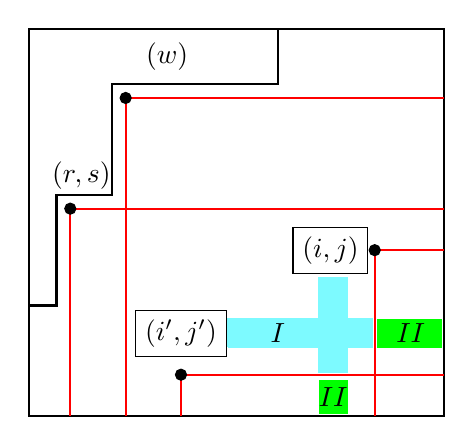
\begin{tikzpicture}[x=2em,y=2em]
      \draw[color=black, thick](0,1)rectangle(7.5,8);
      \draw[color = black, thick](4.5,8)--(4.5,7)--(1.5,7)--(1.5,5)--(0.5,5)--(0.5,3)--(0,3);
     \draw[thick,color=red] (7.5,6.75)--(1.75,6.75)--(1.75,1);
     \draw[thick,color=red] (7.5,4.75)--(0.75,4.75)--(0.75,1);
     \filldraw [black](1.75,6.75)circle(.1);
     \filldraw [black](0.75,4.75)circle(.1);
     \node at (2.5,7.5) {$\Dom(w)$};
     \node at (.95,5.35){$(r,s)$};
     \node[draw] at (5.45,4) {$(i,j)$};
     \node[draw] at (2.75,2.5) {$(i',j')$};																				
   \draw[thick,color=red] (7.5,4)--(6.25,4)--(6.25,1);
     \draw[thick,color=red] (7.5,1.75)--(2.75,1.75)--(2.75,1);
     \filldraw [black](6.25,4)circle(.1);
     \filldraw [black](2.75,1.75)circle(.1);
     \filldraw[color = electricblue, thick](3.6,2.25)--(5.25,2.25)--(5.25,1.8)--(5.75,1.8)--(5.75,2.25)--(6.2,2.25)--(6.2,2.75)--(5.75,2.75)--(5.75,3.5)--(5.25,3.5)--(5.25,2.75)--(3.6,2.75)--(3.6,2.25);
     \node at (4.5,2.5) {$I$};
     \filldraw[color = green](5.25,1.05)rectangle(5.75,1.65);
     \filldraw[color = green](6.3,2.25)rectangle(7.45,2.75);
     \node at (6.9,2.5) {$II$};
      \node at (5.5,1.35) {$II$};
        \end{tikzpicture}.
\]
\end{center}
\end{example}



\begin{lemma}\label{lem:obstruction2}
If the permutation $w \in S_n$ contains an obstruction of Type $2$, then $w$ contains $21543$, $214635$, $241635$, $215364$, or $315264$.
\end{lemma}
\begin{proof}
Fix a permutation $w \in S_n$ that has an obstruction of Type $2$.  We will first assume that we have fixed $(i,j)$ and $(i,j')$ as in the definition of a Type $2$ obstruction with $j'<j$ and $(r,s)$ assumed to be the easternmost element of $\Dom(w) \cap \Ess(w)$ northwest of both $(i,j)$ and $(i,j')$.  As before, we consider the visualization of the Rothe diagram $D_w$.

Label the $\bullet$ in column $s+1$ with $(a,w_a)$ and the $\bullet$ in the row $r+1$ with $(b,w_b)$.  Notice $a<b$ and $w_a>w_b$.  Label the $\bullet$ in row $i$ with $(c,w_c)$, the $\bullet$ in column $j$ with $(d,w_d)$, and the $\bullet$ in column $j'$ with $(e,w_e)$.  If $e>d$, then we have $a<b<c<d<e$ and $w_b<w_a<w_e<w_d<w_c$, which is to say that $w$ contains $21543$.  Now assume $e<d$.  Because $(i',j'), (i,j) \in \Ess(w)$, there must be some $\bullet$ in column $j'+1$, which we label $(f,w_f)$, north of row $i$.  Because of the easternmost assumption on $(r,s)$ and because $\max_k \{(k,j) \in \Dom(w)\} = \max_k \{(k,j') \in \Dom(w)\}$, we must have that $f>a$.  If $f>b>a$, then $w$ contains $214635$ and, if $b>f>a$, then $w$ contains $241635$.  

A parallel argument shows that if $w$ has an obstruction of Type 2 with $i'<i$, $j' = j$, and $\max_\ell \{(i,\ell) \in \Dom(w)\} = \max_\ell \{(i',\ell) \in \Dom(w)\}$, then $w$ contains $21543$, $215364$, or $315264$.
\end{proof}

\begin{lemma}\label{lem:obstruction3}
If the permutation $w \in S_n$ has an obstruction of Type $3$, then $w$ contains $13254$, $21543$, $214635$, $215364$, $215634$, $241635$, $315264$, or $4261735$.  
\end{lemma}

\begin{proof}
Fix a permutation $w \in S_n$ that has an obstruction of Type $3$.  We fix $(i,j)$, $(i',j')$ as in the definition of an obstruction of Type $3$, and consider the visualization of the Rothe diagram of $w$.  If there is some $(r,s) \in \Dom(w) \cap \Ess(w)$ strictly northwest of $(i,j)$, then $w$ has an obstruction of Type $1$,  and so it follows from Lemma \ref{lem:obstruction1} that $w$ contains $21543$, $215634$, $215364$, $214635$, or $13254$.  Hence, we assume no such $(r,s)$ exists.  Without loss of generality, we assume that the $\bullet$ in row $1$ is west of column $j'$ and that the $\bullet$ in column $1$ is north of row $i'$.  

First suppose that the $\bullet$ in row $1$ is west of column $j$.  Then the assumption that there is no $(r,s) \in \Dom(w) \cap \Ess(w)$ strictly northwest of $(i,j)$ implies that the $\bullet$ in column $1$ is south of row $i$.  Because $(i,j) \in \Ess(w)$, there must be a $\bullet$ in column $j+1$ weakly north of row $i$.  If the $\bullet$ in column $j$ is north of row $i'$, then the $\bullet$s in row $1$ and columns $j$ and $j+1$ combine with the $\bullet$s in row $i'$ and column $j'$ to form $13254$.  If the $\bullet$ in column $j$ is south of the $\bullet$ in column $j'$, then they combine with the $\bullet$s in row $1$, column $1$, and row $i'$ to form $21543$.  And if the $\bullet$ in column $j$ is north of the $\bullet$ in column $j'$ but south of row $i'$, then all $\bullet$s described in this paragraph form $241635$. 

Alternatively, assume that the $\bullet$ in row $1$ is between columns $j$ and $j'$.  If the $\bullet$ in column $1$ is north of row $i$, then taking transposes in the argument in the previous paragraph shows that $w$ must contain $13254$, $21543$, or $315264$.  

If the $\bullet$ in column $1$ is south of row $i$, label the $\bullet$ in row $1$ with $(a, w_a)$, any fixed $\bullet$ northwest of $(i,j)$ with $(b, w_b)$, and the $\bullet$ in column $1$ with $(c,w_c)$.  We know that there is some $\bullet$ northwest of $(i,j)$ because $(i,j) \notin \Dom(w)$.  As before, if the $\bullet$ in row $i$ is west of column $j'$ and the $\bullet$ in column $j$ is north of row $i'$, then $w$ contains $13254$.  

Suppose that the $\bullet$ in row $i$ is east of column $j'$, and label that $\bullet$ with $(d,w_d)$.  Label the $\bullet$ in row $i'$ with $(e,w_e)$, and the $\bullet$ in column $j'$ with $(f,w_f)$.  If $w_e<w_d$, then $(a,w_a)$, $(b,w_b)$, $(d,w_d)$, $(e,w_e)$, and $(f,w_f)$ form $21543$.  If $w_e>w_d$, then we consider the placement of the $\bullet$ in column $j$, which we label $(g,w_g)$.  If $g<e$, then $(a,w_a)$, $(b,w_b)$, $(d,w_d)$, $(e,w_e)$, $(f,w_f)$, and $(g,w_g)$ form $315264$.  If $e>g>f$, then all $\bullet$s $(a,w_a)$ to $(g,w_g)$, form $4261735$.  And if $f<g$, then $(b,w_b)$, $(c,w_c)$, $(e,w_e)$, $(f,w_f)$, and $(g,w_g)$ form $21543$.  

Finally, the cases in which $w_d<w_f$ (equivalently, the $\bullet$ in row $i$ west of column $j'$) and $g<e$ are achieved by taking the transpose of the configurations in the preceding paragraph.  In these cases, $w$ contains $21543$, $241635$, or $4261735$.
\end{proof}

\subsection{Permutations avoiding the specified patterns are CDG} \label{subsect:backward} The remainder of this section is devoted to the backward direction of Conjecture \ref{conj:mainresult}.  We will build up to a use of \cite[Corollary 4.13]{KR}.  We begin with some notation.

If $I_w$ is the Schubert determinantal ideal of the permutation $w \in S_n$, we will use $Z_w$ to denote the matrix obtained from an $n \times n$ matrix of indeterminates by setting $z_{i,j}$ to $0$ whenever $(i,j) \in \Dom(w)$.   If $(i,j)$ is a lower outside corner of $D_w$ and $y = z_{i,j}$, we write the CDG generators of $I_w$ as $\{yq_1+r_1, \ldots, yq_k+r_k, h_1, \ldots, h_\ell\}$ where $y$ does not divide any term of any $q_i$, $r_i$ or $h_j$.  Define $N_{y,I_w} = (h_1, \ldots, h_\ell)$ and $C_{y,I_w} = (q_1, \ldots, q_k, h_1, \ldots, h_\ell)$.  This notation mimics that in \cite{KR}.  When the CDG generators are a Gr\"obner basis of $I_w$, $C_{y,I_w}$ will be the ideal corresponding to the star and $N_{y,I_w}+(y)$ the ideal corresponding to the deletion in a geometric vertex decomposition in the sense of \cite{KMY09}.

We will call $\{q_1, \ldots, q_k, h_1, \ldots, h_\ell\}$ the \emph{CDG generators} of $C_{y,I_w}$, which is itself not typically a Schubert determinantal ideal.  With notation as above, we begin by showing that $N_{y,I_w}$ is the Schubert determinantal ideal of a permutation whose Coxeter length is smaller than that of $w$, which will be an essential component of an inductive argument.

Let $t_{a,b}$ denote the transposition $(ab) \in S_n$.

\begin{lemma}\label{lem:SchubertDel}
Suppose that $I_w$ is the Schubert determinantal ideal of the permutation $w \in S_n$ and that $(i,j)$ is a lower outside corner of $D_w$ corresponding to the variable $y = z_{i,j}$.  The ideal $N_{y,I_w}$ is the Schubert determinantal ideal of a permutation $w' \in S_n$ whose Coxeter length is strictly smaller than that of $w$.  Specifically, $w' = wt_{i,w^{-1}(j)}$, and $D_w = D_{w'} \sqcup \{(i,j)\}$.  
\end{lemma}
\begin{proof}
We claim that whenever there is some $(\rank_w(i,j)+1)$-minor with $yq+r = r$, that $r \in N_{y,I_w}$, i.e. that all of the CDG generators of $I_w$ determined only by the rank condition at $(i,j)$ involve $y$.  Fix a $(\rank_w(i,j)+1) \times (\rank_w(i,j)+1)$ submatrix $M$ of $Z_w$ so that $\det(M) = yq+r$, and suppose that $q = 0$.  Recall that the entry in row $a$ and column $b$ of $M$ is $0$ if and only if $(a,b) \in \Dom(w)$.  Then $q$ is the determinant of a $\rank_w(i,j) \times \rank_w(i,j)$ submatrix of $M$ whose anti-diagonal has an entry in row $a$ and column $b$ for some $(a,b) \in \Dom(w)$.  Assume without loss of generality that $i \geq j$.  

If $r \neq 0$, then there is some $(i',j)$ with nonvanishing $z_{i',j} \cdot q'$  summand of $r$ so that $q'$ is the determinant of a $\rank_w(i,j) \times \rank_w(i,j)$ submatrix of $M$ without a $0$ along its anti-diagonal.  Because $\Dom(w)$ forms a partition shape, if $z_{i',j}\cdot q' \neq 0$, then $z_{i'',j} \cdot q'' \neq 0$ whenever $i''<i'$ and $q''$ is the cofactor corresponding to $z_{i'',j}$ in an expansion of $yq+r$ along column $j$.  In particular, there is a unique $t$ so that no $\rank_w(i,j) \times \rank_w(i,j)$ submatrix of $M$ that excludes column $j$ and involves the final $t$ rows has a $0$ along its anti-diagonal and every $\rank_w(i,j) \times \rank_w(i,j)$ submatrix of $M$ that excludes column $j$ and also excludes one of the final $t$ rows has a $0$ along its anti-diagonal.  

The same argument can be applied to columns, and, because vanishing is determined by $0$'s along the anti-diagonal, will select the final $\rank_w(i.j)+1-t$ columns.  Hence, we may write  $r$ as the product of one $t$-minor determined by the final $t$ rows and initial $t$ columns of $M$ and one $(\rank_w(i.j)+1-t)$-minor consisting of the initial $\rank_w(i.j)+1-t$ rows and final $\rank_w(i.j)+1-t$ columns of $M$.  

Call the southeast corner of the lower block $z$ and the southeast corner of the upper block $z'$.  If there are fewer than $t$ dots northwest of $z$, then the $t$-minor that is one factor of $r$ is an element of $N_{y,I_w}$, and so $r \in  N_{y,I_w}$.  If there are $t$ or more dots northwest of $z$, then there are at most $\rank_w(i.j)-t$ dots northwest of $z'$, and so the factor of $r$ corresponding to the upper block is an element of $N_{y,I_w}$, and so $r \in N_{y,I_w}$.  Hence, $N_{y,I_w}$ is generated by the CDG generators of $I_w$ determined by the diagram boxes other than $(i,j)$.  The permutation with exactly those diagram boxes and rank conditions at those diagram boxes is $w' = wt_{i,w^{-1}(j)}$.  Then $N_{y,I_w} = I_{w'}$, the Coxeter length of $w'$ is one less than the Coxeter length of $w$, and $D_w = D_{w'} \sqcup \{(i,j)\}$.  
\end{proof}

\begin{example}
With notation as in Lemma \ref{lem:SchubertDel}, let $w = 215634$ and $(i,j) = (4,4)$.  If $t_{i,w^{-1}(j)} = t_{4,6}$, set $w' = wt_{4,6} = 215436$.  The Rothe diagrams of $w$ and $w'$ appear below.  We may view the Rothe diagram of $w'$ as arising from the Rothe diagram of $w$ by swapping rows $i=4$ and $w^{-1}(j)=6$.  This exchange eliminates the diagram box in position $(i,j) = (4,4)$ and leaves the rest of the diagram boxes undisturbed.

\[
 \begin{minipage}{.4\textwidth}
\hspace{0.5cm} 
  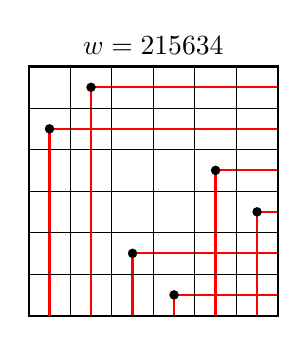
\begin{tikzpicture}[x=1.5em,y=1.5em]
      \draw[color=black, thick](0,1)rectangle(6,7);
           \node at (3,7.5) {$w = 215634$};
     \draw[color=black](0,6)rectangle(1,7);
      \draw[color=black](1,6)rectangle(2,7);
      \draw[color=black](1,4)rectangle(2,5);
      \draw[color=black](3,4)rectangle(4,5);
       \draw[color=black](1,3)rectangle(2,4);
      \draw[color=black](3,3)rectangle(4,4);
      \draw[color=black](1,2)rectangle(2,3);      
     \draw[thick,color=red] (6,6.5)--(1.5,6.5)--(1.5,1);
     \draw[thick,color=red] (6,5.5)--(0.5,5.5)--(0.5,1);
     \draw[thick,color=red] (6,4.5)--(4.5,4.5)--(4.5,1);
     \draw[thick,color=red] (6,3.5)--(5.5,3.5)--(5.5,1);
     \draw[thick,color=red] (6,2.5)--(2.5,2.5)--(2.5,1);
     \draw[thick,color=red] (6,1.5)--(3.5,1.5)--(3.5,1);
     \filldraw [black](1.5,6.5)circle(.1);
     \filldraw [black](0.5,5.5)circle(.1);
      \filldraw [black](4.5,4.5)circle(.1);
     \filldraw [black](5.5,3.5)circle(.1);
     \filldraw [black](2.5,2.5)circle(.1);
      \filldraw [black](3.5,1.5)circle(.1);
      \draw[color=black](2,6)rectangle(3,7);
      \draw[color=black](3,6)rectangle(4,7); 
      \draw[color=black](4,6)rectangle(5,7);
      \draw[color=black](5,6)rectangle(6,7); 
      \draw[color=black](0,5)rectangle(1,6);
      \draw[color=black](1,5)rectangle(2,6);  
      \draw[color=black](2,5)rectangle(3,6);
      \draw[color=black](3,5)rectangle(4,6); 
      \draw[color=black](4,5)rectangle(5,6);
      \draw[color=black](5,5)rectangle(6,6); 
     \draw[color=black](0,4)rectangle(1,5); 
      \draw[color=black](2,4)rectangle(3,5);
      \draw[color=black](4,4)rectangle(5,5);
      \draw[color=black](5,4)rectangle(6,5); 
      \draw[color=black](0,3)rectangle(1,4); 
      \draw[color=black](2,3)rectangle(3,4);
      \draw[color=black](4,3)rectangle(5,4);
      \draw[color=black](5,3)rectangle(6,4); 
      \draw[color=black](0,2)rectangle(1,3); 
      \draw[color=black](2,2)rectangle(3,3);
      \draw[color=black](3,2)rectangle(4,3);
      \draw[color=black](4,2)rectangle(5,3);
      \draw[color=black](5,2)rectangle(6,3); 
      \draw[color=black](1,1)rectangle(2,2);  
      \draw[color=black](2,1)rectangle(3,2);
      \draw[color=black](3,1)rectangle(4,2); 
      \draw[color=black](4,1)rectangle(5,2);
      \draw[color=black](5,1)rectangle(6,2); 
     \end{tikzpicture}
  \end{minipage}    \begin{minipage}{.4\textwidth}
\hspace{1cm} 
  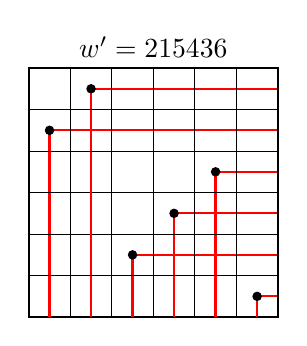
\begin{tikzpicture}[x=1.5em,y=1.5em]
      \draw[color=black, thick](0,1)rectangle(6,7);
           \node at (3,7.5) {$w' =215436 $};
     \draw[color=black](0,6)rectangle(1,7);
      \draw[color=black](1,6)rectangle(2,7);
      \draw[color=black](1,4)rectangle(2,5);
      \draw[color=black](3,4)rectangle(4,5);
       \draw[color=black](1,3)rectangle(2,4);
      \draw[color=black](3,3)rectangle(4,4);
      \draw[color=black](1,2)rectangle(2,3);      
     \draw[thick,color=red] (6,6.5)--(1.5,6.5)--(1.5,1);
     \draw[thick,color=red] (6,5.5)--(0.5,5.5)--(0.5,1);
     \draw[thick,color=red] (6,4.5)--(4.5,4.5)--(4.5,1);
     \draw[thick,color=red] (6,3.5)--(3.5,3.5)--(3.5,1);
     \draw[thick,color=red] (6,2.5)--(2.5,2.5)--(2.5,1);
     \draw[thick,color=red] (6,1.5)--(5.5,1.5)--(5.5,1);
     \filldraw [black](1.5,6.5)circle(.1);
     \filldraw [black](0.5,5.5)circle(.1);
      \filldraw [black](4.5,4.5)circle(.1);
     \filldraw [black](3.5,3.5)circle(.1);
     \filldraw [black](2.5,2.5)circle(.1);
      \filldraw [black](5.5,1.5)circle(.1);
      \draw[color=black](2,6)rectangle(3,7);
      \draw[color=black](3,6)rectangle(4,7); 
      \draw[color=black](4,6)rectangle(5,7);
      \draw[color=black](5,6)rectangle(6,7); 
      \draw[color=black](0,5)rectangle(1,6);
      \draw[color=black](1,5)rectangle(2,6);  
      \draw[color=black](2,5)rectangle(3,6);
      \draw[color=black](3,5)rectangle(4,6); 
      \draw[color=black](4,5)rectangle(5,6);
      \draw[color=black](5,5)rectangle(6,6); 
     \draw[color=black](0,4)rectangle(1,5); 
      \draw[color=black](2,4)rectangle(3,5);
      \draw[color=black](4,4)rectangle(5,5);
      \draw[color=black](5,4)rectangle(6,5); 
      \draw[color=black](0,3)rectangle(1,4); 
      \draw[color=black](2,3)rectangle(3,4);
      \draw[color=black](4,3)rectangle(5,4);
      \draw[color=black](5,3)rectangle(6,4); 
      \draw[color=black](0,2)rectangle(1,3); 
      \draw[color=black](2,2)rectangle(3,3);
      \draw[color=black](3,2)rectangle(4,3);
      \draw[color=black](4,2)rectangle(5,3);
      \draw[color=black](5,2)rectangle(6,3); 
      \draw[color=black](1,1)rectangle(2,2);  
      \draw[color=black](2,1)rectangle(3,2);
      \draw[color=black](3,1)rectangle(4,2); 
      \draw[color=black](4,1)rectangle(5,2);
      \draw[color=black](5,1)rectangle(6,2); 
     \end{tikzpicture}.
  \end{minipage}   
       \]
\end{example}

\begin{remark}\label{rem:newEss}
With notation as in Lemma \ref{lem:SchubertDel}, it is possible that $\Ess(w') \not\subseteq \Ess(w)$, as is the case if $w = 215634$ and $(i,j) = (4,4)$.  In that case, $(3,4), (4,3) \in \Ess(w') \setminus \Ess(w)$.  

In general, the only possible elements of $\Ess(w') \setminus \Ess(w)$ are $(i-1,j)$ and $(i,j-1)$.  Indeed, suppose $(a,b) \in \Ess(w') \setminus \Ess(w)$. By the definition of $\Ess(w')$, $(a,b) \in D_{w'}$ and $(a+1,b), (a,b+1) \notin D_{w'}$.  Because $D_{w'} \subset D_w$, the assumption $(a,b) \notin \Ess(w)$ implies $(a+1,b) \in \Ess(w)$ or $(a,b+1) \in \Ess(w)$.  The fact that $D_w \setminus D_{w'} = \{(i,j)\}$ then implies that $(a+1,b) = (i,j)$ or $(a,b+1) = (i,j)$.
\end{remark}

\begin{corollary}\label{cor:GrobnerDel}
If $w$ has no obstruction of Type $1$, $2$, or $3$, $(i,j)$ is a lower outside corner of $D_w$ corresponding to the variable $y = z_{i,j}$, and $I_{w'} =N_{y,I_w}$, then $w'$ has no obstruction of Type $1$, $2$, or $3$.  
\end{corollary}

\begin{proof}
If $(i,j) \in \Dom(w)$, then, because there are no diagram boxes southeast of $(i,j)$ by assumption, $(i,j)$ cannot be one of the boxes involved in any of the obstructions.  In that case, any set of diagram boxes realizing an obstruction in $w'$ would also realize an obstruction in $w$.  Hence we assume that $(i,j) \notin \Dom(w)$, in which case $\Dom(w) = \Dom(w')$.

Suppose that $w'$ has an obstruction of Type $1$ with $(r,s) \in \Dom(w') \cap \Ess(w')$ and $(a,b)$, $(a'b') \in D_{w'}$ strictly southeast of $(r,s)$ with $a' \neq a$ and $b' \neq b$.  Because $\Dom(w') = \Dom(w)$ and $D_{w'} \subset D_w$, the diagram boxes $(r,s)$, $(a,b)$, $(a',b')$ also constitute an obstruction of Type $1$ in $w$ as well.

Next suppose that $w'$ has an obstruction of Type $2$.  Assume without loss of generality that the Type $2$ obstruction has the form  $(r,s) \in \Dom(w') \cap \Ess(w')$ and $(a,b), (a,b') \in \Ess(w')$ strictly southeast of $(r,s)$ with $\max_k \{(k,b) \in \Dom(w')\} = \max_k \{(k,b') \in \Dom(w') \}$ and $b<b'$.  In this case neither $(a,b)$ nor $(r,s)$ may be a lower outside corner of $w'$.   In particular, neither $(r,s)$ nor $(a,b)$ is equal to $(i,j)$, and so $(r,s) \in \Dom(w) \cap \Ess(w)$ and $(a,b) \in \Ess(w)$.  If $(a,b') \in \Ess(w)$ also, then $(r,s)$, $(a,b)$, and $(a,b')$ also constitute a Type $2$ obstruction in $w$.  If $(a,b') \notin \Ess(w)$, then either $(a+1,b') = (i,j) \in \Ess_w$, in which case $(r,s)$, $(a,b)$, and $(a+1,b')$ together constitute a Type $1$ obstruction, or $(a,b'+1) = (i,j) \in \Ess(w)$.  

If $(a,b'+1) = (i,j) \in \Ess(w)$, set $m = \max_k \{(k,b) \in \Dom(w')\} = \max_k \{(k,b') \in \Dom(w')\}$.  Because $\Dom(w) = \Dom(w')$, we have $m = \max_k \{(k,b) \in \Dom(w)\}$.  We claim that $m = \max_k \{(k,b'+1) \in \Dom(w)\}$.   Because $b'+1>b'$ and $\Dom(w)$ forms a partition shape, $m \geq \max_k \{(k,b'+1) \in \Dom(w)\}$.  If $m > \max_k \{(k,b'+1) \in \Dom(w)\}$, then $(m,b'+1) \notin \Dom(w)$.  But $(m,b') \in \Dom(w') = \Dom(w)$.  Therefore, if $(m,b'+1) \notin \Dom(w)$, the visualization of $D_w$ must have a $\bullet$ in column $b'+1$ weakly north of row $m$.  Clearly $m<a$ since $(a,b) \notin \Dom(w')$.  But the $\bullet$ in column $b'+1 = j$ must be south of row $a = i$ because $(i,j) \in D_w$. Hence, $m = \max_k \{(k,b'+1) \in \Dom(w)\}$ and $(r,s)$, $(a,b)$, and $(a, b'+1)$ together constitute a Type $3$ obstruction in $w$. 

Finally suppose that $w'$ has an obstruction of Types $3$.  Suppose that $(a,b), (a',b') \in \Ess(w') \setminus \Dom(w')$ with $(a',b')$ strictly southeast of $(a,b)$.  If $(a',b') \in \Ess(w)$, then $(a,b)$ and $(a',b')$ constitute a Type $3$ obstruction in $w$ also.  Otherwise, it must be that $(i,j) = (a'+1,b')$ or $(i,j) = (a',b+1)$.  In either case, $(a,b)$ and $(i,j)$ constitute a Type $3$ obstruction in $w$.
\end{proof}

Next, we will show that the CDG generators of $C_{y,I_w}$ form a Gr\"obner basis whenever $w$ has no obstruction of Type $1$, $2$, or $3$.  Before proceeding, we review some standard notation and make one new definition to help with bookkeeping during this subsection.  We will use $\deg(f)$ to denote the degree of the homogeneous polynomial $f$ and $LCM(\mu_1,\mu_2)$ to denote the least common multiple of two monomials (which will arise for us as the monic leading terms of ideal generators).  

\begin{definition}\label{def:Qdef}
Fix a permutation $w \in S_n$, lower outside corner $(i,j)$ of $D_w$ corresponding to the variable $y = z_{i,j}$ in $Z_w$, and CDG generators $\{yq_1+r_1, \ldots, yq_k+r_k, h_1, \ldots, h_\ell \}$ of $I_w$, where $y$ does not divide any $q_a$, $r_a$, or $h_b$.  Assume also that there is some $0 \leq \ell' \leq \ell$ so that all variables appearing in $h_b$ are northwest of some $z_{i',j}$ for $(i',j) \in \Ess(w)$ with $\rank_w(i',j) +1= \deg(h_b)$ or of some $z_{i,j'}$ for $(i,j') \in \Ess(w)$ with $\rank_w(i,j') +1= \deg(h_b)$ if and only if $b \leq \ell'$.  If $(1,j) \in \Dom(w)$, set $m_1 = \min\{i-p \mid (p,j) \in \Dom(w)\}$, and set $m_1 = i$ if $(1,j) \notin \Dom(w)$.  Similarly, if $(i,1) \in \Dom(w)$, set $m_2 = \min\{j-q \mid (i,q) \in \Dom(w)\}$, and set $m_2 = j$ if $(1,j) \notin \Dom(w)$. 

We form the ideal \[ Q_{y,I_w} = \begin{cases} 
      (q_1, \ldots, q_k) & \rank_w(i,j)+1 = \min\{m_1,m_2\} \\
     (q_1, \ldots, q_k, h_1, \ldots, h_{\ell'}) & \mbox{otherwise}. \\
   \end{cases}
\]
\end{definition}

Less formally, we are taking $Q_{y,I_w} = (q_1, \ldots, q_k)$ when the rank condition on $(i,j)$ is determining maximal minors in the submatrix of $Z_w$ obtained from the submatrix northwest of $z_{i,j}$ by deleting any full rows or columns of $0$'s.  Otherwise, we include also as generators of $Q_{y,I_w}$ the CDG generators determined by essential boxes in the same row or column as $z_{i,j}$.  

\begin{example}
Let $w = 351624$ and $y = z_{4,4}$.  The Rothe diagram of $w$ is \[
  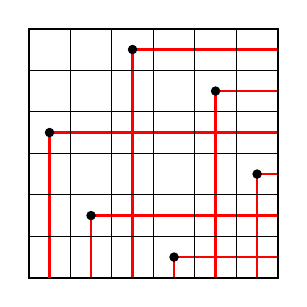
\begin{tikzpicture}[x=1.5em,y=1.5em]
      \draw[color=black, thick](0,1)rectangle(6,7);
      \draw[color=black](1,4)rectangle(2,5);
      \draw[color=black](3,4)rectangle(4,5);
       \draw[color=black](1,3)rectangle(2,4);
      \draw[color=black](3,3)rectangle(4,4);
      \draw[color=black](1,2)rectangle(2,3);
      \draw[color=black](0,1)rectangle(1,2);  
     \draw[thick,color=red] (6,6.5)--(2.5,6.5)--(2.5,1);      
     \draw[thick,color=red] (6,5.5)--(4.5,5.5)--(4.5,1);
     \draw[thick,color=red] (6,4.5)--(0.5,4.5)--(0.5,1);
     \draw[thick,color=red] (6,3.5)--(5.5,3.5)--(5.5,1);
     \draw[thick,color=red] (6,2.5)--(1.5,2.5)--(1.5,1);
     \draw[thick,color=red] (6,1.5)--(3.5,1.5)--(3.5,1);
     \filldraw [black](0.5,4.5)circle(.1);
      \filldraw [black](5.5,3.5)circle(.1);
     \filldraw [black](4.5,5.5)circle(.1);
     \filldraw [black](3.5,1.5)circle(.1);
      \filldraw [black](1.5,2.5)circle(.1);
      \filldraw [black](2.5,6.5)circle(.1);
      \draw[color=black](0,6)rectangle(1,7);
      \draw[color=black](1,6)rectangle(2,7);  
      \draw[color=black](2,6)rectangle(3,7);
      \draw[color=black](3,6)rectangle(4,7); 
      \draw[color=black](4,6)rectangle(5,7);
      \draw[color=black](5,6)rectangle(6,7);
      \draw[color=black](0,5)rectangle(1,6);
      \draw[color=black](1,5)rectangle(2,6);  
      \draw[color=black](2,5)rectangle(3,6);
      \draw[color=black](3,5)rectangle(4,6); 
      \draw[color=black](4,5)rectangle(5,6);
      \draw[color=black](5,5)rectangle(6,6);
     \draw[color=black](0,4)rectangle(1,5); 
      \draw[color=black](2,4)rectangle(3,5);
      \draw[color=black](4,4)rectangle(5,5);
      \draw[color=black](5,4)rectangle(6,5);
      \draw[color=black](0,3)rectangle(1,4); 
      \draw[color=black](2,3)rectangle(3,4);
      \draw[color=black](4,3)rectangle(5,4);
      \draw[color=black](5,3)rectangle(6,4);
      \draw[color=black](0,2)rectangle(1,3); 
      \draw[color=black](2,2)rectangle(3,3);
      \draw[color=black](3,2)rectangle(4,3);
      \draw[color=black](4,2)rectangle(5,3);
      \draw[color=black](5,2)rectangle(6,3);
      \draw[color=black](1,1)rectangle(2,2);  
      \draw[color=black](2,1)rectangle(3,2);
      \draw[color=black](3,1)rectangle(4,2); 
      \draw[color=black](4,1)rectangle(5,2);
      \draw[color=black](5,1)rectangle(6,2);
     \end{tikzpicture}.
\] 
Then \[
I_w = (z_{1,1}, z_{1,2}, z_{2,1}, z_{2,2}, 2\text{-minors in } (Z_w)_{[4],[2]},  2\text{-minors in } (Z_w)_{[2],[4]}, 3\text{-minors in } (Z_w)_{[4],[4]})
\] and  \[
Q_{y,I_w} = (2\text{-minors in } (Z_w)_{[4],[2]},  2\text{-minors in } (Z_w)_{[2],[4]}, 2\text{-minors in } (Z_w)_{[3],[3]}).
\] The $2$-minors in $(Z_w)_{[2],[4]}$, for example, are included as generators of $Q_{y,I_w}$ because \[
\rank_w(4,4)+1 = 3<4 = \min\{4,4\} = \min\{m_1,m_2\}
\] and $(2,4) \in \Ess(w)$ is in the same column as $(4,4)$.  
\end{example}

We make this definition purely for technical convenience below and not out of an independent interest in $\Spec(R/Q_{y,I_w})$.  We will say that $Q_{y,I_w}$ is CDG if the generators given above form a Gr\"obner basis under any diagonal term order.  

\begin{lemma}\label{lem:GrobnerQs}
If $w \in S_n$ has no obstruction of Type $1$, $2$, or $3$ and Conjecture \ref{conj:mainresult} holds for all permutations of smaller Coxeter length than that of $w$, then either $D_w = \Dom(w)$ or there is some lower outside corner $(i,j)$ of $D_w \setminus \Dom(w)$ corresponding to the variable $y$ in $Z_w$ so that $Q_{y,I_w}$ is CDG.
\end{lemma}
\begin{proof}
Fix a permutation $w \in S_n$ that has no obstruction of Type $1$, $2$, or $3$, and assume $D_w \neq \Dom(w)$.  First suppose that $D_w$ has some lower outside corner $(i,j)\notin \Dom(w)$ corresponding to the variable $y$ in $Z_w$ satisfying $\rank_w(i,j)+1 = \min\{m_1,m_2\}$, with notation as in Definition \ref{def:Qdef}.  

Write the CDG generators of $I$ as $\{yq_1+r_1, \ldots, yq_k+r_k, h_1, \ldots, h_\ell \}$, where $y$ does not divide any $q_i$, $r_i$, or $h_j$.  As discussed in Lemma \ref{lem:SchubertDel}, every $(\rank_w(i,j)+1)$-minor involving row $i$ and column $j$ has a term divisible by $y$, and so $\{q_1, \ldots, q_k\}$ generates the ideal of $\rank_w(i,j)$-minors in the submatrix of $Z_w$ strictly northwest of $y$.  Because the $Q_{y,I}$ is an ideal of maximal minors (after possible removing full rows or columns of $0$'s), the result follows from \cite[Theorem 4.2]{CDG15} or \cite[Proposition 5.4]{Boo11}.  

Alternatively, suppose that $D_w$ has no such lower outside corner, and fix any lower outside corner of $D_w$.  Because $Q_{y,I_w}$ depends only on $D_w$ weakly northwest of $(i,j)$, we may assume that $(i,j)$ is the only lower outside corner of $D_w$ and that $(1,j), (i,1) \notin \Dom(w)$.  With this assumption, $Q_{y,I_w} +(z_{a,b} \mid (a,b) \in \Dom(w))= C_{y,I_w}$.  Because the $z_{a,b}$ with $(a,b) \in \Dom(w)$ are indeterminates that do not divide any term of any CDG generator of $Q_{y,I_w}$, it follows that $Q_{y,I_w}$ is CDG if and only if $C_{y,I_w}$ is CDG.  

If $\Dom(w) = \emptyset$, then, because $w$ has no obstruction of Type $1$, $w$ must be vexillary and so $I_w$ is CDG by \cite[Theorem 3.8]{KMY09}.   It then follows from  \cite[Theorem 2.1(a)]{KMY09} that $C_{y,I_w}$ is CDG as well.  

Now suppose $\Dom(w) \neq \emptyset$.  The assumptions that $(1,j), (i,1) \notin \Dom(w)$ imply that there is at least one element of $\Dom(w) \cap \Ess(w)$ northwest of $(i,j)$.  Choose the southernmost such element and label it $(r,s)$ and the easternmost element and label it $(r',s')$.  Because $w$ has no obstruction of Type $1$, all essential boxes of $D_w \setminus \Dom(w)$ must be in either row $i$ or column $j$.  Because $\rank_w(i,j)+1 < \min\{i,j\}$, there must be at least one essential box in row $i$ and at least one in column $j$ aside from $(i,j)$. Then because $w$ has no obstruction of Type $2$, there are no elements of $\Ess(w)$ north of row $i$ and south of row $r$ or west of column $j$ and east of column $s'$.  

We will argue directly in this case that for each pair $q_a$ and $h_b$, their $s$-polynomial has a Gr\"obner reduction by the CDG generators of $Q_{y,I_w}$.  (For an example illustrating this process, see Example \ref{ex:Spoly} below.)  Choose such a $q_a$ and $h_b$.  Because the CDG generators of $N_{y,I_w}$ form a Gr\"obner basis by induction on the Coxeter length of $w$ and Corollary \ref{cor:GrobnerDel}, we may assume that $q_a \notin (h_1, \ldots, h_\ell)$.  

Because $Q_{y,I_w}$ involves only indeterminates of $Z_w$ northwest of $z_{i,j}$, we will work within the submatrix of $Z_w$ northwest of $z_{i,j}$, which we will call $Y_w$.  Suppose that $h_b$ is determined by the essential box at $(i',j)$ for some $i'<i$.  (The case of $(i,j')$ with $j'<j$ will follow by symmetry.)  We consider two cases.  

Case 1: Suppose that $(i',j-1) \in D_w$.  Then, because $w$ has no obstruction of Type $1$, there can be no element of $\Dom(w) \cap \Ess(w)$ northwest of $(i',j)$.  In particular, $r' \geq i'$, and $h_b$ is a $(\rank_w(i',j)+1)$-minor in the submatrix of $Y_w$ formed of its final $j-s'$ columns, which is a generic matrix and which we will call $Y'_w$.  Suppose that there are $t$ columns determining $q_a$ strictly east of column $s'$ and $\rank_w(i,j)-t$ columns determining $q_a$ weakly west of column $s'$.  Express $q_a$ as a sum of products of $t$-minors and $(\rank_w(i,j)-t)$-minors corresponding to this subdivision.  For any fixed set of rows of $Y'_w$, the set of $(\rank_w(i',j)+1)$-minors weakly northwest of $(i',j)$ together with the $t$-minors strictly northwest of $(i,j)$ in the submatrix of $Y'_w$ including only those specified rows forms a Gr\"obner basis for the ideal they generate because it is a mixed ladder determinantal ideal \cite[Theorem 1.10]{Gor07}.  

Choose the $t$-minor $\varepsilon_1$ from the eastern $t$ columns determining $q_a$ and the $(\rank_w(i,j)-t)$-minor $\varepsilon_2$ from the remaining columns satisfying $LT(\varepsilon_1) \cdot LT(\varepsilon_2) = LT(q_a)$.  Because $\varepsilon_1$ and $h_b$ belong to the ideal of $t$-minors weakly north of their southernmost entries together with the $(\rank_w(i',j)+1)$-minors northwest of $(i',j)$ in $Y'_w$, their $s$-polynomial $s(\varepsilon_1,h_b)$ has a Gr\"obner reduction $s(\varepsilon_1,h_b) = \sum \alpha_c \delta_c $ by the natural generators of that ideal.  For each $\delta_c \in N_{y,I_w}$, set $\widehat{\delta_c} = LT(\varepsilon_2) \cdot \delta_c$, and for each $\delta_c$ involving some row south of $i'$, set $\widehat{\delta_c}$ to be (up to sign) the determinant of the augmentation of the matrix determining $\delta_c$ by the rows and columns determining $\varepsilon_2$ (with sign chosen so that $LT(\delta_c)$ and $LT(\widehat{\delta_c})$ share a sign).  Let $s(q_a,h_b)$ denote the $s$-polynomial of $q_a$ and $h_b$.  

We claim that $s(q_a,h_b)-\sum \alpha_c \widehat{\delta_c} \in N_{y,I}$.  It is clear that $s(q_a,h_b)-\sum \alpha_c \widehat{\delta_c}$ contains a $LT(\varepsilon_2)$-multiple of $s(\varepsilon_1,h_b)-\sum \alpha_c \delta_c$, which is $0$ because $s(\varepsilon_1,h_b)-\sum \alpha_c \delta_c$ is.  Fix any non-leading term $\mu$ of $\varepsilon_2$, and write $s(q_a,h_b)-\sum \alpha_c \widehat{\delta_c} = \mu \tilde{s}+\tilde{\tilde{s}}$ where $\mu$ does not divide any term of $\tilde{\tilde{s}}$.  For each column involved in $\varepsilon_2$, whenever a different variable from that column divides $\mu$ and $LT(\varepsilon_2)$, replace in $\sum \alpha_c \widehat{\delta_c}$ the variables in the row of the divisor of $LT(\varepsilon_2)$ with the variables in the same columns from the row of the corresponding divisor of $\mu$, which we note gives an expression of $\tilde{s}$ in terms of the natural generators of the ideal of $(\rank_w(i',j)+1)$-minors northwest of $(i',j)$, each of which is a CDG generator of $N_{y,I}$.

Now because $LT(\alpha_c\delta_c) \leq LT(s(\varepsilon_1,h_b))$ and $LT(\alpha_c \widehat{\delta_c}) = LT(\varepsilon_2) \cdot LT(\alpha_c\delta_c)$ for each $c$ and because $LT(s(q_a,h_b)) = LT(\varepsilon_2) \cdot LT(s(\varepsilon_1,h_b))$, subtracting each $\alpha_c \widehat{\delta_c}$ is a valid step in a Gr\"obner reduction of $s(q_a,h_b)$ by the generators of $Q_{y,I_w}$.  The fact that the CDG generators of $N_{y,I_w}$, each of which is a CDG generator of $Q_{y,I_w}$, form a Gr\"obner basis for the ideal they generate implies that $s(q_a,h_b)-\sum \alpha_c \widehat{\delta_c} \in N_{y,I_w}$ has a reduction in terms of those generators and so that $s(q_a,h_b)$ has a reduction by the CDG generators of $Q_{y,I_w}$.

Case 2: Suppose $(i',j-1) \notin D_w$.  Then there can be no $j''<j$ with $(i',j'') \in D_w\setminus \Dom(w)$ because $w$ has no obstruction of Type $3$.  Hence, $\rank_w(i',j)+1 = \min\{j-k \mid (i',k) \in \Dom(w)\}$, and so the $(\rank_w(i',j)+1)$-minors northwest of $(i',j)$ are the maximal minors of the submatrix of $Z_w$ northwest of $(i',j)$ after removing complete rows or columns of $0$'s.  Then the argument is similar to the first case but uses, instead of results on ladder determinantal ideals in a generic matrix, the fact that the maximal minors of matrices of indeterminates and $0$'s form a Gr\"obner basis by \cite[Theorem 4.2]{CDG15} or \cite[Proposition 5.4]{Boo11}.  
\end{proof}

\begin{example}\label{ex:Spoly}
Observe that $w = 378149256$, whose annotated Rothe diagram appears below, is an example of a CDG permutation with a unique lower outside corner  $(i,j) = (6,6)$ and $4=\rank_w(i,j)+1 \neq \min\{m_1,m_2\}=6$.  We illustrate how the reduction of the $s$-polynomial of $h_b = \begin{vmatrix} z_{2,3} & z_{2,4} \\ z_{3,3} & z_{3,4} \end{vmatrix}$ and $\begin{vmatrix} z_{2,3} & z_{2,5} \\ z_{5,3} & z_{5,5} \end{vmatrix}$ gives rise to that of $\begin{vmatrix} z_{2,3} & z_{2,4} \\ z_{3,3} & z_{3,4} \end{vmatrix}$ and $q_a = \begin{vmatrix} 0 & z_{2,3} & z_{2,5} \\ z_{4,2} & z_{4,3} & z_{4,5} \\ z_{5,2} & z_{5,3} & z_{5,5} \end{vmatrix}$ by the process described in Lemma \ref{lem:GrobnerQs}.  Using that \[
z_{5,5} { \color{burntorange}\begin{vmatrix} z_{2,3} & z_{2,4} \\ z_{3,3} & z_{3,4} \end{vmatrix}}-z_{3,4} \begin{vmatrix} z_{2,3} & z_{2,5} \\ z_{5,3} & z_{5,5} \end{vmatrix} +z_{2,4} \begin{vmatrix} z_{3,3} & z_{3,5} \\ z_{5,3} & z_{5,5} \end{vmatrix} + z_{5,3} {\color{burntorange} \begin{vmatrix} z_{2,4} & z_{2,5} \\ z_{3,4} & z_{3,5} \end{vmatrix}} = 0,
\] we construct the equation \begin{align*}
 {\color{blue}\underline{z_{4,2} z_{5,5} \begin{vmatrix} z_{2,3} & z_{2,4} \\ z_{3,3} & z_{3,4} \end{vmatrix}}}+{\color{blue}\underline{z_{3,4}} }\begin{vmatrix} 0 & \color{blue}\underline{z_{2,3}} & \color{blue}\underline{z_{2,5}} \\ \color{blue}\underline{z_{4,2}} & z_{4,3} & z_{4,5} \\  z_{5,2} & \color{blue}\underline{z_{5,3}} & \color{blue}\underline{z_{5,5}} \end{vmatrix}  &- 
  {\color{blue}\underline{z_{2,4}}} \begin{vmatrix} 0 & \color{blue}\underline{z_{3,3}} & \color{blue}\underline{z_{3,5}} \\ \color{blue}\underline{z_{4,2}} & z_{4,3} & z_{4,5} \\ z_{5,2} & \color{blue}\underline{z_{5,3}} & \color{blue}\underline{z_{5,5}} \end{vmatrix}+ {\color{blue}\underline{z_{4,2} z_{5,3} \begin{vmatrix} z_{2,4} & z_{2,5} \\ z_{3,4} & z_{3,5} \end{vmatrix} }}\\
  &= z_{5,2} \left(z_{4,5}   {\color{burntorange}\begin{vmatrix} z_{2,3} & z_{2,4} \\ z_{3,3} & z_{3,4} \end{vmatrix}} +z_{4,3} { \color{burntorange} \begin{vmatrix} z_{2,4} & z_{2,5} \\ z_{3,4} & z_{3,5} \end{vmatrix}}\right).
\end{align*} In the latter equation, we find an $z_{4,2}$-multiple of the first equation (whose terms appear in blue and also are underlined) and an $z_{5,2}$-multiple of an element easily seen to be in $N_{y,I_w}$.  We record in orange the generators of $N_{y,I_w}$ that give the inclusion of the $z_{5,2}$-multiple summand of $s(q_a,h_b)$ in $N_{y,I_w}$ and see that relation arising from the first equation.  The new relation is obtained from the first by exchanging rows $4$ and $5$.  
\[
\hspace{1cm} 
\hspace{0.5cm} 
  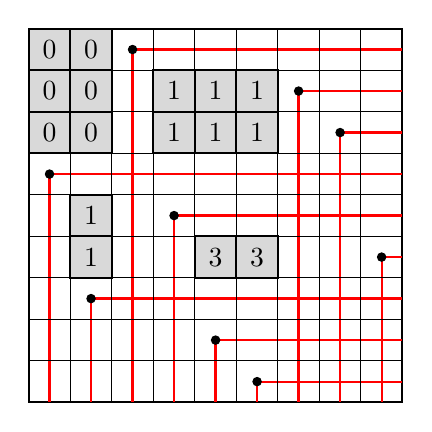
\begin{tikzpicture}[x=1.5em,y=1.5em]
      \draw[color=black, thick](0,1)rectangle(9,10);
     \filldraw[color=black, fill=gray!30, thick](0,9)rectangle(1,10);
      \filldraw[color=black, fill=gray!30, thick](1,9)rectangle(2,10);
      \filldraw[color=black, fill=gray!30, thick](0,7)rectangle(1,8);
      \filldraw[color=black, fill=gray!30, thick](0,8)rectangle(1,9);
      \filldraw[color=black, fill=gray!30, thick](1,8)rectangle(2,9);
      \filldraw[color=black, fill=gray!30, thick](1,7)rectangle(2,8);
      \filldraw[color=black, fill=gray!30, thick](1,4)rectangle(2,5);
     \filldraw[color=black, fill=gray!30, thick](1,5)rectangle(2,6);
      \filldraw[color=black, fill=gray!30, thick](5,4)rectangle(6,5);
       \draw[color=black](1,3)rectangle(2,4);
      \draw[color=black](3,3)rectangle(4,4);  
     \draw[thick,color=red] (9,9.5)--(2.5,9.5)--(2.5,1);
     \draw[thick,color=red] (9,8.5)--(6.5,8.5)--(6.5,1);
     \draw[thick,color=red] (9,5.5)--(3.5,5.5)--(3.5,1);
     \draw[thick,color=red] (9,1.5)--(5.5,1.5)--(5.5,1);
     \draw[thick,color=red] (9,7.5)--(7.5,7.5)--(7.5,1);
     \draw[thick,color=red] (9,2.5)--(4.5,2.5)--(4.5,1);
     \draw[thick,color=red] (9,3.5)--(1.5,3.5)--(1.5,1);
     \draw[thick,color=red] (9,6.5)--(0.5,6.5)--(0.5,1);
     \draw[thick,color=red] (9,4.5)--(8.5,4.5)--(8.5,1);
     \filldraw [black](2.5,9.5)circle(.1);
     \filldraw [black](6.5,8.5)circle(.1);
     \filldraw [black](0.5,6.5)circle(.1);
      \filldraw [black](5.5,1.5)circle(.1);
     \filldraw [black](7.5,7.5)circle(.1);
     \filldraw [black](4.5,2.5)circle(.1);
      \filldraw [black](1.5,3.5)circle(.1);
      \filldraw [black](3.5,5.5)circle(.1);
      \filldraw [black](8.5,4.5)circle(.1);
       \draw[color=black](2,7)rectangle(3,8);
      \filldraw[color=black, fill=gray!30, thick](3,7)rectangle(4,8); 
      \filldraw[color=black, fill=gray!30, thick](4,7)rectangle(5,8);
      \filldraw[color=black, fill=gray!30, thick](5,7)rectangle(6,8); 
      \filldraw[color=black, fill=gray!30, thick](5,8)rectangle(6,9);
      \draw[color=black](5,7)rectangle(6,8); 
     \draw[color=black](2,8)rectangle(3,9);
      \draw[color=black](3,8)rectangle(4,9); 
      \draw[color=black](4,8)rectangle(5,9);
      \draw[color=black](5,8)rectangle(6,9); 
      \draw[color=black](2,6)rectangle(3,7);
      \draw[color=black](0,1)rectangle(1,2);
      \draw[color=black](1,2)rectangle(2,3);
      \draw[color=black](3,4)rectangle(4,5);
      \draw[color=black](1,6)rectangle(2,7);
      \draw[color=black](2,6)rectangle(3,7);
      \filldraw[color=black, fill=gray!30, thick](3,8)rectangle(4,9); 
      \filldraw[color=black, fill=gray!30, thick](4,8)rectangle(5,9);
      \draw[color=black](5,6)rectangle(6,7); 
      \draw[color=black](0,5)rectangle(1,6);
      \draw[color=black](1,5)rectangle(2,6);  
      \draw[color=black](2,5)rectangle(3,6);
      \draw[color=black](3,5)rectangle(4,6); 
      \draw[color=black](4,5)rectangle(5,6);
      \draw[color=black](5,5)rectangle(6,6); 
     \draw[color=black](0,4)rectangle(1,5); 
      \draw[color=black](2,4)rectangle(3,5);
    \filldraw[color=black, fill=gray!30, thick](4,4)rectangle(5,5);
      \draw[color=black](5,4)rectangle(6,5); 
      \draw[color=black](0,3)rectangle(1,4); 
      \draw[color=black](2,3)rectangle(3,4);
      \draw[color=black](4,3)rectangle(5,4);
      \draw[color=black](5,3)rectangle(6,4); 
      \draw[color=black](0,2)rectangle(1,3); 
      \draw[color=black](2,2)rectangle(3,3);
      \draw[color=black](3,2)rectangle(4,3);
      \draw[color=black](4,2)rectangle(5,3);
      \draw[color=black](5,2)rectangle(6,3); 
      \draw[color=black](1,1)rectangle(2,2);  
      \draw[color=black](0,6)rectangle(1,7);  
      \draw[color=black](0,9)rectangle(1,10); 
      \draw[color=black](1,9)rectangle(2,10); 
      \draw[color=black](2,1)rectangle(3,2);
      \draw[color=black](2,9)rectangle(3,10); 
      \draw[color=black](3,1)rectangle(4,2); 
      \draw[color=black](3,9)rectangle(4,10); 
      \draw[color=black](4,1)rectangle(5,2);
      \draw[color=black](4,9)rectangle(5,10); 
      \draw[color=black](5,1)rectangle(6,2); 
      \draw[color=black](5,9)rectangle(6,10); 
      \draw[color=black](6,1)rectangle(7,2); 
      \draw[color=black](6,2)rectangle(7,3); 
      \draw[color=black](6,3)rectangle(7,4); 
      \draw[color=black](6,4)rectangle(7,5); 
      \draw[color=black](6,5)rectangle(7,6); 
      \draw[color=black](6,6)rectangle(7,7); 
      \draw[color=black](6,7)rectangle(7,8); 
      \draw[color=black](6,8)rectangle(7,9);
      \draw[color=black](6,9)rectangle(7,10);  
       \draw[color=black](7,1)rectangle(8,2); 
      \draw[color=black](7,2)rectangle(8,3); 
      \draw[color=black](7,3)rectangle(8,4); 
      \draw[color=black](7,4)rectangle(8,5); 
      \draw[color=black](7,5)rectangle(8,6); 
      \draw[color=black](7,6)rectangle(8,7); 
      \draw[color=black](7,7)rectangle(8,8); 
      \draw[color=black](7,8)rectangle(8,9);
       \draw[color=black](7,9)rectangle(8,10);  
      \draw[color=black](8,1)rectangle(9,2); 
      \draw[color=black](8,2)rectangle(9,3); 
      \draw[color=black](8,3)rectangle(9,4); 
      \draw[color=black](8,4)rectangle(9,5); 
      \draw[color=black](8,5)rectangle(9,6); 
      \draw[color=black](8,6)rectangle(9,7); 
      \draw[color=black](8,7)rectangle(9,8); 
      \draw[color=black](8,8)rectangle(9,9); 
      \draw[color=black](8,9)rectangle(9,10); 
      \draw[color=black](4,5)rectangle(6,7); 
      \node at (0.5,9.5) {$0$};
      \node at (1.5,9.5) {$0$};
      \node at (0.5,7.5) {$0$};
     \node at (1.5,7.5) {$0$};
      \node at (0.5,8.5) {$0$};
      \node at (1.5,8.5) {$0$};
      \node at (1.5,4.5) {$1$};
       \node at (1.5,5.5) {$1$};
       \node at (5.5,4.5) {$3$};
       \node at (4.5,4.5) {$3$};
       \node at (3.5,8.5) {$1$};
       \node at (4.5,8.5) {$1$};
       \node at (3.5,7.5) {$1$};
       \node at (4.5,7.5) {$1$};
       \node at (5.5,7.5) {$1$};
       \node at (5.5,8.5) {$1$};
     \end{tikzpicture}.
       \]
\end{example}

Before proceeding, we recall one very useful lemma.

\begin{lemma}\label{lem:concatinate}\cite[Lemma 1.3.14]{Con93}
Let $I$ and $J$  be  homogeneous ideals of a polynomial ring over a field, and fix a term order $\sigma$.  With respect to $\sigma$, let  $\mathcal{F}$  be  a  Gr\"obner basis of $I$ and $\mathcal{G}$ a Gr\"obner basis of $J$.  Then $\mathcal{F} \cup \mathcal{G}$ is a Gr\"obner basis of $I+J$ if and only if for all $f \in \mathcal{F}$ and $g \in \mathcal{G}$ there exists $e \in I \cap J$ such that $LT(e) = LCM(LT(f),LT(g))$. \qed
\end{lemma}

We are now prepared to show that, under a suitable inductive hypothesis, there is a lower outside corner so that the CDG generators of $C_{y,I_w}$ are Gr\"obner.

\begin{lemma}\label{lem:GrobnerLink}
With notation as above, if $w \in S_n$ avoids obstructions of Types $1$, $2$, and $3$ and Conjecture \ref{conj:mainresult} holds for all permutations of smaller Coxeter length than that of $w$, then either $D_w = \Dom(w)$ or there is some lower outside corner $(i,j)$ of $D_w \setminus \Dom(w)$ corresponding to the variable $y = z_{i,j}$ so that the generators $\{q_1, \ldots, q_k, h_1, \ldots, h_\ell\}$ of $C_{y,I_w}$ form a Gr\"obner basis under any diagonal term order.
\end{lemma}
\begin{proof}
Fix a diagonal term order $\sigma$, and assume $D_w \neq \Dom(w)$.  By Lemma \ref{lem:GrobnerQs}, there is some lower outside corner of $D_w$ so that, with notation as above, there exists $\ell' \geq 0$ so that the generators $\{q_1, \ldots, q_k, h_1, \ldots, h_{\ell'} \}$ form a Gr\"obner basis for $Q_{y,I_w}$.  

By Corollary \ref{cor:GrobnerDel} and the inductive hypothesis, $\{h_1,\ldots, h_\ell\}$ is a diagonal Gr\"obner basis for $N_{y,I_w}$.  Then by Lemma \ref{lem:concatinate}, the generators $\{q_1, \ldots, q_k, h_1, \ldots, h_\ell\}$ form a diagonal Gr\"obner basis for $C_{y,I_w}$ if and only if for every $q_a$ and $h_b$ there exists some $f \in (q_1, \ldots, q_k, h_1, \ldots, h_{\ell'}) \cap (h_1, \ldots, h_\ell)$ satisfying $LT(f) = LCM(LT(q_a),LT(h_b))$.  

If $h_b \in (q_1, \ldots, q_k, h_1, \ldots, h_{\ell'})$ or $q_a \in (h_1, \ldots, h_\ell)$, the result follows from Lemma \ref{lem:concatinate}, and if $LCM(LT(q_a),LT(h_b)) = LT(q_a) \cdot LT(h_b)$, then we take $f = q_a \cdot h_b$.  Otherwise, there is some $(r,s) \in \Ess(w) \setminus \Dom(m)$ with $\rank_w(r,s) = \deg(h_b)-1$ corresponding to the variable $e = z_{r,s}$ weakly southeast of all of the variables involved in $h_b$.  Because $w$ has no Type $3$ obstruction, $e$ is not strictly northwest of $y$.  Suppose first that $y$ is strictly east and weakly north of $e$.

In this case, let $M'$ be the matrix consisting of the union of the columns determining $q_a$ and $h_b$ and the union of the rows determining $q_a$ and $h_b$.  We will next describe an auxiliary matrix $M$ formed from $M'$. (For an example of the construction, see Example \ref{ex:formM} below.)  Form a matrix $M$ from $M'$ as follows: First set to $0$ any entry whose row index is not one of the rows determining $q_a$ and whose column index is not one of the columns determining $h_b$.  Next, whenever a column of $M'$ contains a variable dividing the leading term of $q_a$ and a distinct variable dividing the leading term of $h_b$, duplicate that column and replace in one copy of the column the variables coming only from $h_b$ by $0$.  Whenever a row of $M'$ contains a variable dividing the leading term of $q_a$ and a distinct variable dividing the leading term of $h_b$, duplicate that row and replace in one copy of the row the variables coming only from $q_a$ by $0$.  

Now $M$ will be a $d \times d$ matrix where $d = \deg(LCM(LT(q_a),LT(h_b)))$ because it will have one row and one column for each monomial dividing $LT(q_a)$ and one each for every monomial dividing $LT(h_b)$ but not $LT(q_a)$.  

By expressing $\det(M)$ as a sum of products of the $\deg(q_a)$-minors from the rows of $M$ originating from the submatrix of $Z_w$ determining $q_a$ and the $(d-\deg(q_a))$-minors in the remaining rows, we see that $\det(M) \in (q_1, \ldots, q_k)$.  Similarly, by expressing $\det(M)$ as a sum of products of $\deg(h_b)$-minors in the column originating from the submatrix of $Z_w$ determining from $h_b$ and $(d-\deg(h_b))$-minors in the remaining columns, we have $\det(M) \in (h_1, \ldots, h_\ell)$.  It is because $y$ is strictly east and weakly north of $e$ that the rows determining $q_a$ that every $\deg(q_a)$-minor in the specified rows is an element of $(q_1, \ldots, q_k)$ and that every $\deg(h_b)$-minor in the specified column is an element of $(h_1, \ldots, h_\ell)$.

Next we will see that $LT(\det(M)) = LCM(LT(q_a),LT(h_b))$.  Call $\tilde{M}$ the submatrix of $M'$ whose entries are northwest of both $e$ and $y$.  Set $\mu_1$ to be the product of the terms of $\tilde{M}$ that divide either $LT(q_a)$ or $LT(h_b)$.  Call $\mu_2$ the leading term of the determinant of the submatrix of $M$ consisting of the rows and columns used to determine $h_b$ excluding those involving a divisor of $\mu_1$.  Similarly, define $\mu_3$ to be the leading term of the determinant of the submatrix of $M$ consisting of the rows and columns determining $q_a$ excluding those involving a divisor of $\mu_1$.  

Notice that $\mu_1 \cdot \mu_2 \cdot \mu_3 = LCM(LT(q_a),LT(h_b))$ and that this product is a term of $\det(M)$.  To see that every other term of $\det(M)$ is smaller under $\sigma$, notice that because $w$ has no obstruction of Type $1$, the submatrix of $M'$ whose entries are both northwest of $e$ and northwest of $y$ must have $0$'s only in full rows and full columns along the north and west sides.  

It will now be more convenient for us to work with $\widehat{M}$, obtained from $M$ by adding the doubled copies of rows and columns obtained in the transition from $M'$ to $M$ so that no variable appears more than once.  Note that $\det(\widehat{M}) = \det(M)$.  If some other term of $\det(\widehat{M})$ is larger than $\mu_1 \cdot \mu_2 \cdot \mu_3$, there must be some entries of $\widehat{M}$ dividing $\mu_1 \cdot \mu_2 \cdot \mu_3$ whose row indices we may permute to obtain a larger monomial.  We may assume that this permutation consists of one cycle.  If all entries divide either $\mu_1 \cdot \mu_2$ or $\mu_1\cdot \mu_3$, we would obtain a term of $q_a$ or $h_b$, respectively, that is strictly larger than its leading term, which also cannot be.  But the permutation cannot send any divisor of $\mu_3$ to the row of a divisor of $\mu_1$, all of which are $0$ in that column, or vice versa.  Hence, $\mu_1 \cdot \mu_2 \cdot \mu_3 = LT(\det(\widehat{M})) = LT(\det(M))$, as desired.

Finally, if $y$ is strictly south and weakly west of $e$, a parallel argument gives the~result.
\end{proof}

\begin{example}\label{ex:formM}
Below we give an example of the construction of the matrices $M'$ and $M$.  Let $w = 5237164$, $y = z_{4,6}$, \[
q_a = \det \begin{bmatrix} 0& 0 & {\color{blue}\underline{z_{1,5}}}\\
{\color{blue}\underline{z_{2,2}}} & z_{2,3} & z_{2,5}\\
z_{3,2}& {\color{blue}\underline{z_{3,3}}} & z_{3,5}
 \end{bmatrix} \in Q_{y, I_w}, \mbox{ and } h_b = \det \begin{bmatrix} 
 0 & {\color{blue}\underline{z_{2,2}}} & z_{2,3} & z_{2,4} \\
0 & z_{4,2} & {\color{blue}\underline{z_{4,3}}} & z_{4,4} \\
{ \color{blue} \underline{z_{5,1}}} & z_{5,2} & z_{5,3} & z_{5,4} \\
  z_{6,1} & z_{6,2} & z_{6,3} & {\color{blue}\underline{z_{6,4}}} \\
 \end{bmatrix} \in N_{y,I_w},
 \] in which case $LT(q_a) = z_{1,5}z_{2,2}z_{3,3}$, $LT(h_b) = z_{2,2}z_{4,3}z_{5,1}z_{6,4}$, and \[ 
 LCM(LT(q_a),LT(h_b)) = z_{1,5}z_{2,2}z_{3,3}z_{4,3}z_{5,1}z_{6,4} = LT(\det(M)).
 \]  The variables dividing the leading terms appearing throughout this example are noted in blue and also underlined.  Then \[
 M' = \begin{bmatrix} 
 0 & 0 & 0 & 0 & {\color{blue}\underline{z_{1,5}}}\\
 0 & {\color{blue}\underline{z_{2,2}}} & z_{2,3} & z_{2,4} & z_{2,5}\\
  0 & z_{3,2} & {\color{blue}\underline{z_{3,3}}} & z_{3,4} & z_{3,5}\\
0 & z_{4,2} & {\color{blue}\underline{z_{4,3}}} & z_{4,4} & z_{4,5}\\
  {\color{blue}\underline{z_{5,1}}} & z_{5,2} & z_{5,3} & z_{5,4} & z_{5,5} \\
  z_{6,1} & z_{6,2} & z_{6,3} &  {\color{blue}\underline{z_{6,4}}} & z_{6,5} 
 \end{bmatrix} \mbox{  \hspace{0.5cm}   and  \hspace{0.5cm}   } M  = \begin{bmatrix} 
 0 & 0 & 0 & 0 & 0 & {\color{blue}\underline{z_{1,5}}}\\
 0 & {\color{blue}\underline{z_{2,2}}} & z_{2,3} & z_{2,3} & z_{2,4} & z_{2,5}\\
  0 & z_{3,2} & {\color{blue}\underline{z_{3,3}}} & {\color{blue}\underline{z_{3,3}}} & z_{3,4} & z_{3,5}\\
0 & z_{4,2} & 0 & {\color{blue}\underline{z_{4,3}}}  & z_{4,4} & 0\\
  {\color{blue}\underline{z_{5,1}}} & z_{5,2} & 0 & z_{5,3} & z_{5,4} &0 \\
  z_{6,1} & z_{6,2} & 0  & z_{6,3}& {\color{blue}\underline{z_{6,4}}}  & 0
 \end{bmatrix}.
 \] 

 By expressing $\det(M)$ as a sum of products of $3$-minors in the first $3$ rows of $M$ with $3$-minors in the final $3$ rows, we see $\det(M) \in Q_{y,I_w}$, and, by expressing $\det(M)$ as the sum of products of $4$-minors in columns $1$, $2$, $4$, and $5$ with $2$-minors in columns $3$ and $6$, we see $\det(M) \in N_{y,I_w}$.  Observe that \begin{align*}
 LT(\det(M)) &=  LT\left(\det \begin{bmatrix} z_{2,2} & z_{2,3} \\ z_{3,2} & z_{3,3} \end{bmatrix} \right) \cdot LT\left(\det  \begin{bmatrix} 0 & z_{4,3} & z_{4,4} \\ z_{5,1} & z_{5,3} & z_{5,4} \\ z_{6,1} & z_{6,3} & z_{6,4} \end{bmatrix}\right) \cdot z_{1,5} \cdot\\
 &= (z_{2,2}z_{3,3})(z_{4,3}z_{5,1}z_{6,4})(z_{1,5}).
 \end{align*}
 This expression corresponds to the product $\mu_1 \cdot \mu_2 \cdot \mu_3$ in the proof of Lemma \ref{lem:GrobnerLink}.  One may prefer to use $\widehat{M}$, as in the lemma, obtained from $M$ by subtracting column $3$ from column $4$, which has the effect of setting the copies of $z_{2,3}$ and $z_{3,3}$ in column $4$ to $0$.  
 
One aspect of this example that is typical of the general case is that the intersection of the submatrix of of $M'$ northwest of $z_{6,4}$ (playing the role of $e$) and that northwest of $z_{3,5}$ (from $z_{4,6}$ playing the role of $y$) is a rectangular matrix of indeterminates with $0$'s appearing only in full rows along the top and full columns along the western side of the submatrix.  This arrangement follows from the fact that $5237164$ has no obstruction of Type $1$ and gives rise to the decomposition of $LT(\det(M))$ described above into a product of the leading term of entries along the main diagonal of a matrix of indeterminates together with entries coming only from $q_a$ and entries coming only from $h_b$.
\end{example}

We are now prepared to use our lemmas above that establish Gr\"obner bases for $N_{y,I_w}$ and $C_{y,I_w}$ by induction to give the backward direction of Conjecture \ref{conj:mainresult}.  We recall a lemma that structures our proof below.  This lemma gives an implementation of the strategy employed throughout \cite{GMN13}.  

\begin{lemma}\label{lem:mainApp}\cite[Corollary 4.13]{KR}.  
Let $I = ( yq_1+r_1,\dots, yq_k+r_k,h_1,\dots, h_\ell )$ be a homogenous ideal of the polynomial ring $R$ with $y$ some variable of $R$ and $y$ not dividing any term of any $q_i$ nor any term of any $h_j$. Fix a term order $\sigma$ satisfying $LT(yq_i+r_i) = yLT(q_i)$ for each $i$.   Suppose that $\mathcal{G}_C = \{q_1,\dots, q_k,h_1,\dots, h_\ell\}$ and $\mathcal{G}_N = \{h_1,\dots, h_\ell\}$ are Gr\"obner bases for the ideals they generate, which we call $C$ and $N$, respectively, and that $\hgt(I)$, $\hgt(C)>\hgt(N)$.  Assume that $N$ has no embedded primes, and let $M = \begin{pmatrix}
q_1& \cdots & q_k\\
r_1& \cdots & r_k
\end{pmatrix}.$ If the ideal of $2$-minors of $M$ is contained in $N$, then the given generators of $I$ are a Gr\"obner basis.
\end{lemma}

\begin{theorem}\label{thm:if}
If $w \in S_n$ is a permutation that has no obstruction of Type $1$, Type  $2$, or Type $3$, then $w$ is CDG.
\end{theorem}

\begin{proof}
Fix a diagonal term order $\sigma$.  We proceed by induction on the Coxeter length of $w$, with the case of length $0$ trivial.  Fix a permutation $w \in S_n$ with $n$ arbitrary and assume that $w$ has no obstruction of Type $1$, Type  $2$, or Type $3$.  If $D_w = \Dom(w)$, then $I_w$ is generated by variables, and so the result is immediate.  Hence, we assume $\Dom(w) \neq D_w$.

According to Lemma \ref{lem:GrobnerLink}, there is some lower outside corner $(i,j)$ of $D_w \setminus \Dom(w)$ corresponding to the variable $y = z_{i,j}$ so that, with our usual notation, $\{yq_1+r_1,\dots, yq_k+r_k,h_1,\dots, h_\ell\}$ are the CDG generators of $I_w$, the generators $\{q_1, \ldots, q_k, h_1, \ldots, h_\ell\}$ of $C_{y,I_w}$ form a Gr\"obner basis, and $LT(yq_a+r_a) = yLT(q_a)$ for each $a$.  By Corollary \ref{cor:GrobnerDel} and the inductive hypothesis, $\{h_1, \ldots, h_\ell\}$ is a Gr\"obner basis for $N_{y,I_w}$.  

We will show that $I_2 \begin{pmatrix} q_1 & \ldots & q_k \\ r_1 & \ldots & r_k \end{pmatrix} \subseteq  N_{y,I}$.  For each CDG generator, $yq_a+r_a$, let $yq_a'+r_a'$ be the corresponding natural generator of $I_w$, i.e. the generator taken in a matrix of indeterminates in which the variables corresponding to $\Dom(w)$ have not been set to $0$.  Let $J = (z_{i,j} \mid (i,j) \in \Dom(w))$.  Then $I_2 \begin{pmatrix} q_1 & \ldots & q_k \\ r_1 & \ldots & r_k \end{pmatrix}+J= I_2 \begin{pmatrix} q_1' & \ldots & q_k' \\ r_1' & \ldots & r_k' \end{pmatrix}+J$.  Hence, because $J \subseteq N_{y,I_w}$, it suffices to show $I_2 \begin{pmatrix} q_1' & \ldots & q_k' \\ r_1' & \ldots & r_k' \end{pmatrix} \subseteq N_{y,I_w}$.  

In order to show this last containment, we will temporarily consider a possibly different diagonal term order $\sigma'$, which will be a lexicographic term order in which $y$ is largest.  It is because $y$ is a lower outside corner that there must exist a term order that is both diagonal and is also lexicographic with $y$ largest.  Now because each $q'_ar'_b-q'_br'_a = (yq'_a+r'_a)q'_b-(yq'_b+r'_b)q'_a$ for $1 \leq a<b \leq k$ is an element of the ideal of  $(\rank_w(i,j)+1)$-minors in a matrix of indeterminates weakly northwest of $y$, an ideal for which the natural generators form a Gr\"obner basis under $\sigma'$ because it is a diagonal order, we know that $q'_ar'_b-q'_br'_a$ has a Gr\"obner reduction in terms of those generators.  Because $q'_ar'_b-q'_br'_a$ does not involve $y$ and $y$ is lexicographically largest under $\sigma'$, that reduction must be in terms of $(\rank_w(i,j)+1)$-minors weakly northwest of $y$ that do not involve $y$.  Each such minor is an element of $N_{y,I_w}$.  Hence, \[
I_2 \begin{pmatrix} q_1 & \ldots & q_k \\ r_1 & \ldots & r_k \end{pmatrix}+J = I_2 \begin{pmatrix} q_1' & \ldots & q_k' \\ r_1' & \ldots & r_k' \end{pmatrix}+J \subseteq N_{y,I_w},
\] as desired. 

The height requirements $\hgt{I_w}, \hgt{C_{y,I_w}} > \hgt{N_{y,I_w}}$ are immediate from the fact that $N_{y,I_w}$ is prime \cite[Proposition 3.3]{Ful92} together with the proper containment of $N_{y,I_w}$ in each of $I_w$ and $C_{y,I_w}$.  The result now follows from Lemma \ref{lem:mainApp}.
\end{proof}

Notice that we do not claim that the Gr\"obner reduction of $q'_ar'_b-q'_br'_a$ with respect to $\sigma'$ gives rise to a Gr\"obner reduction of $a_ar_b-q_br_a$ in terms of the CDG generators with respect to $\sigma$.  Lemma \ref{lem:mainApp} requires only that we demonstrate an ideal containment.
